\documentclass[11pt,a4paper]{article}

% ── Packages ──
\usepackage[utf8]{inputenc}
\usepackage[T1]{fontenc}
\usepackage{fontspec}
\setmainfont{Liberation Sans}
\usepackage[margin=2.5cm]{geometry}
\usepackage{graphicx}
\usepackage{booktabs}
\usepackage{tabularx}
\usepackage{multirow}
\usepackage{caption}
\usepackage{subcaption}
\usepackage{hyperref}
\usepackage{xcolor}
\usepackage{amsmath,amssymb}
\usepackage[super,sort&compress]{natbib}
\usepackage{longtable}
\usepackage{array}
\usepackage{float}
\usepackage{enumitem}

\hypersetup{colorlinks=true, linkcolor=blue, citecolor=blue, urlcolor=blue}

% ── Title ──
\title{Population-referenced multi-omics analysis reveals mineral-pathway dysregulation in spaceflight: \\
       integrating NHANES baseline with astronaut and rodent transcriptomic data from the NASA OSDR}
\author{Richard Barker}
\date{}

\begin{document}

\maketitle

% ════════════════════════════════════════════════════════════════════
% ABSTRACT
% ════════════════════════════════════════════════════════════════════
\begin{abstract}
\noindent
Spaceflight disrupts mineral homeostasis through microgravity-induced bone loss, fluid shifts, and radiation exposure, yet interpreting clinical markers from small astronaut cohorts ($n=4$) lacks population context. We integrated data from the National Health and Nutrition Examination Survey (NHANES, 2013--2018, $n=5{,}748$ adults aged 40--60) as a population reference baseline for 15 clinical mineral and hematological variables, then contextualized measurements from four Inspiration4 astronauts across seven timepoints. Mean platelet volume was significantly elevated above population norms at six of seven timepoints (Benjamini--Hochberg FDR $< 0.05$, Cohen's $d = 2.12$--$2.47$), while calcium ($d = 1.30$--$1.92$) and bicarbonate ($d = -1.24$ to $-1.78$) showed large population-deviating effects. Transcriptomic analysis identified 50 differentially expressed mineral-pathway genes, with copper-dependent enzymes (APP up, LOX/LOXL1 down), iron metabolism genes (ALAS2 down, HFE up), and the calcium channel CACNA1D (down, log$_2$FC $= -2.25$) most affected. Machine learning regression demonstrated that mineral-pathway gene expression predicts serum potassium ($r = 0.50$) and sodium ($r = 0.46$) under leave-one-out cross-validation. A cross-species meta-analysis across 28 rodent datasets revealed significant mineral-pathway concordance in skeletal muscle (pooled $r = 0.035$, $p = 0.0025$), strongest in soleus ($r = 0.059$, $p = 0.009$), but not in liver or kidney. These findings demonstrate that population-referenced framing reveals spaceflight mineral deviations invisible to within-subject analysis alone, with implications for biomarker development and nutritional countermeasures.

\medskip
\noindent\textbf{Keywords:} spaceflight, mineral homeostasis, NHANES, multi-omics, transcriptomics, cross-species meta-analysis, machine learning, Inspiration4, NASA OSDR
\end{abstract}

% ════════════════════════════════════════════════════════════════════
% INTRODUCTION
% ════════════════════════════════════════════════════════════════════
\section{Introduction}

Spaceflight exposes humans to a unique combination of physiological stressors including microgravity, cosmic radiation, confinement, and altered circadian rhythms. These stressors disrupt multiple biological systems\textsuperscript{1}, with mineral homeostasis being particularly vulnerable: microgravity-induced bone resorption releases calcium into the circulation\textsuperscript{11}, cephalad fluid shifts expand central blood volume\textsuperscript{2}, and spaceflight increases oxidative stress\textsuperscript{3}. The NASA Open Science Data Repository (OSDR) provides multi-omics data from the Inspiration4 (I4) mission --- the first all-civilian orbital spaceflight (September 2021, 3-day low-Earth orbit)\textsuperscript{4} --- including RNA-seq, proteomics, metabolomics, and clinical chemistry from four astronauts across seven timepoints.

A fundamental challenge in spaceflight omics research is the extremely small sample size. With $n=4$ astronauts, within-subject comparisons lack the statistical power to distinguish spaceflight-induced changes from normal biological variation. Population reference data can address this limitation by providing an external baseline against which astronaut values can be compared. The National Health and Nutrition Examination Survey (NHANES), conducted by the CDC National Center for Health Statistics, provides nationally representative laboratory data for the U.S. civilian population\textsuperscript{5}, including standard biochemistry profiles and complete blood counts that directly overlap with astronaut clinical measurements.

In this study, we: (1) established NHANES population reference intervals for 15 clinical mineral and hematological variables matched to astronaut data; (2) identified astronaut markers that deviate significantly from population norms; (3) characterized the mineral-pathway transcriptomic response using curated gene sets spanning 10 minerals and 5 KEGG pathways; (4) evaluated whether mineral-pathway gene expression predicts serum mineral levels using machine learning; and (5) conducted a cross-species meta-analysis across 28 rodent datasets to assess translational concordance. By framing astronaut findings within a population baseline, we distinguish population-deviating abnormalities from within-subject variation that may remain within normal physiological ranges.

% ════════════════════════════════════════════════════════════════════
% RESULTS
% ════════════════════════════════════════════════════════════════════
\section{Results}

\subsection{NHANES population reference for clinical mineral markers}

We pooled three consecutive NHANES cycles (2013--2014, 2015--2016, 2017--2018) to construct a stable population reference for 15 clinical variables that directly map to astronaut measurements: five biochemistry analytes (calcium, potassium, sodium, chloride, bicarbonate) from the Standard Biochemistry Profile and ten hematological parameters (hemoglobin, hematocrit, RBC count, MCH, MCHC, MCV, WBC count, RDW, platelet count, MPV) from the Complete Blood Count with 5-part differential. The reference population was restricted to adults aged 40--60 years (all sexes), yielding 5,748 participants (2,713 male, 3,035 female) --- demographically consistent with typical astronaut corps age ranges. Reference intervals (P2.5--P97.5), means, standard deviations, and full percentile distributions were computed for each variable (Table~\ref{tab:nhanes_ref}).

\begin{table}[H]
\centering
\caption{NHANES population reference statistics for key clinical mineral and hematological variables (age 40--60, all sexes, pooled 2013--2018).}
\label{tab:nhanes_ref}
\begin{tabular}{lrlrrr}
\toprule
\textbf{Variable} & \textbf{N} & \textbf{Units} & \textbf{Mean} & \textbf{P2.5} & \textbf{P97.5} \\
\midrule
Calcium & 5,429 & mg/dL & 9.33 & 8.70 & 10.00 \\
Potassium & 5,442 & mmol/L & 3.98 & 3.30 & 4.70 \\
Sodium & 5,444 & mmol/L & 139.48 & 135.00 & 144.00 \\
Chloride & 5,444 & mmol/L & 102.83 & 96.00 & 108.00 \\
Bicarbonate & 5,444 & mmol/L & 25.13 & 21.00 & 30.00 \\
Hemoglobin & 5,519 & g/dL & 14.08 & 10.70 & 16.70 \\
Hematocrit & 5,519 & \% & 41.92 & 33.09 & 49.60 \\
RBC count & 5,519 & M/uL & 4.73 & 3.84 & 5.71 \\
MCH & 5,519 & pg & 29.07 & 22.80 & 33.30 \\
MCHC & 5,519 & g/dL & 33.50 & 31.40 & 35.10 \\
MCV & 5,519 & fL & 88.38 & 70.69 & 98.70 \\
WBC count & 5,519 & 10$^3$/uL & 7.28 & 3.90 & 12.21 \\
RDW & 5,519 & \% & 13.84 & 12.30 & 17.61 \\
Platelet count & 5,519 & 10$^3$/uL & 243.54 & 140.00 & 383.00 \\
MPV & 5,519 & fL & 8.36 & 6.80 & 10.40 \\
\bottomrule
\end{tabular}
\end{table}

\subsection{Astronaut clinical markers deviate from population norms}

Each of the 28 astronaut measurements (4 crew $\times$ 7 timepoints) was converted to a z-score relative to the NHANES age 40--60 reference and evaluated for deviation from the population 95\% reference interval (P2.5--P97.5). One-sample $t$-tests and Wilcoxon signed-rank tests were performed at each timepoint, with Benjamini--Hochberg FDR correction across all 105 tests (15 variables $\times$ 7 timepoints). Three implausible values in one crew member (C003 at L-92: MPV = 330 fL, RDW = 32.4\%, platelet count = 12.9 $\times$ 10$^3$/uL) were identified as data entry errors and excluded.

Mean platelet volume (MPV) was significantly elevated above the NHANES population mean at six of seven timepoints (FDR $< 0.05$; Cohen's $d$ ranging from 2.12 to 2.47); at L-92, where only three crew were measured, the elevation was smaller and not significant after correction ($d = 1.73$, FDR $= 0.13$), with 48.1\% of astronaut MPV measurements falling outside the population 95\% reference interval (Figure~\ref{fig:zscore_heatmap}). This deviation was persistent across pre-flight, flight, and post-flight phases, suggesting a crew-level characteristic rather than a spaceflight-induced shift.

\begin{figure}[H]
\centering
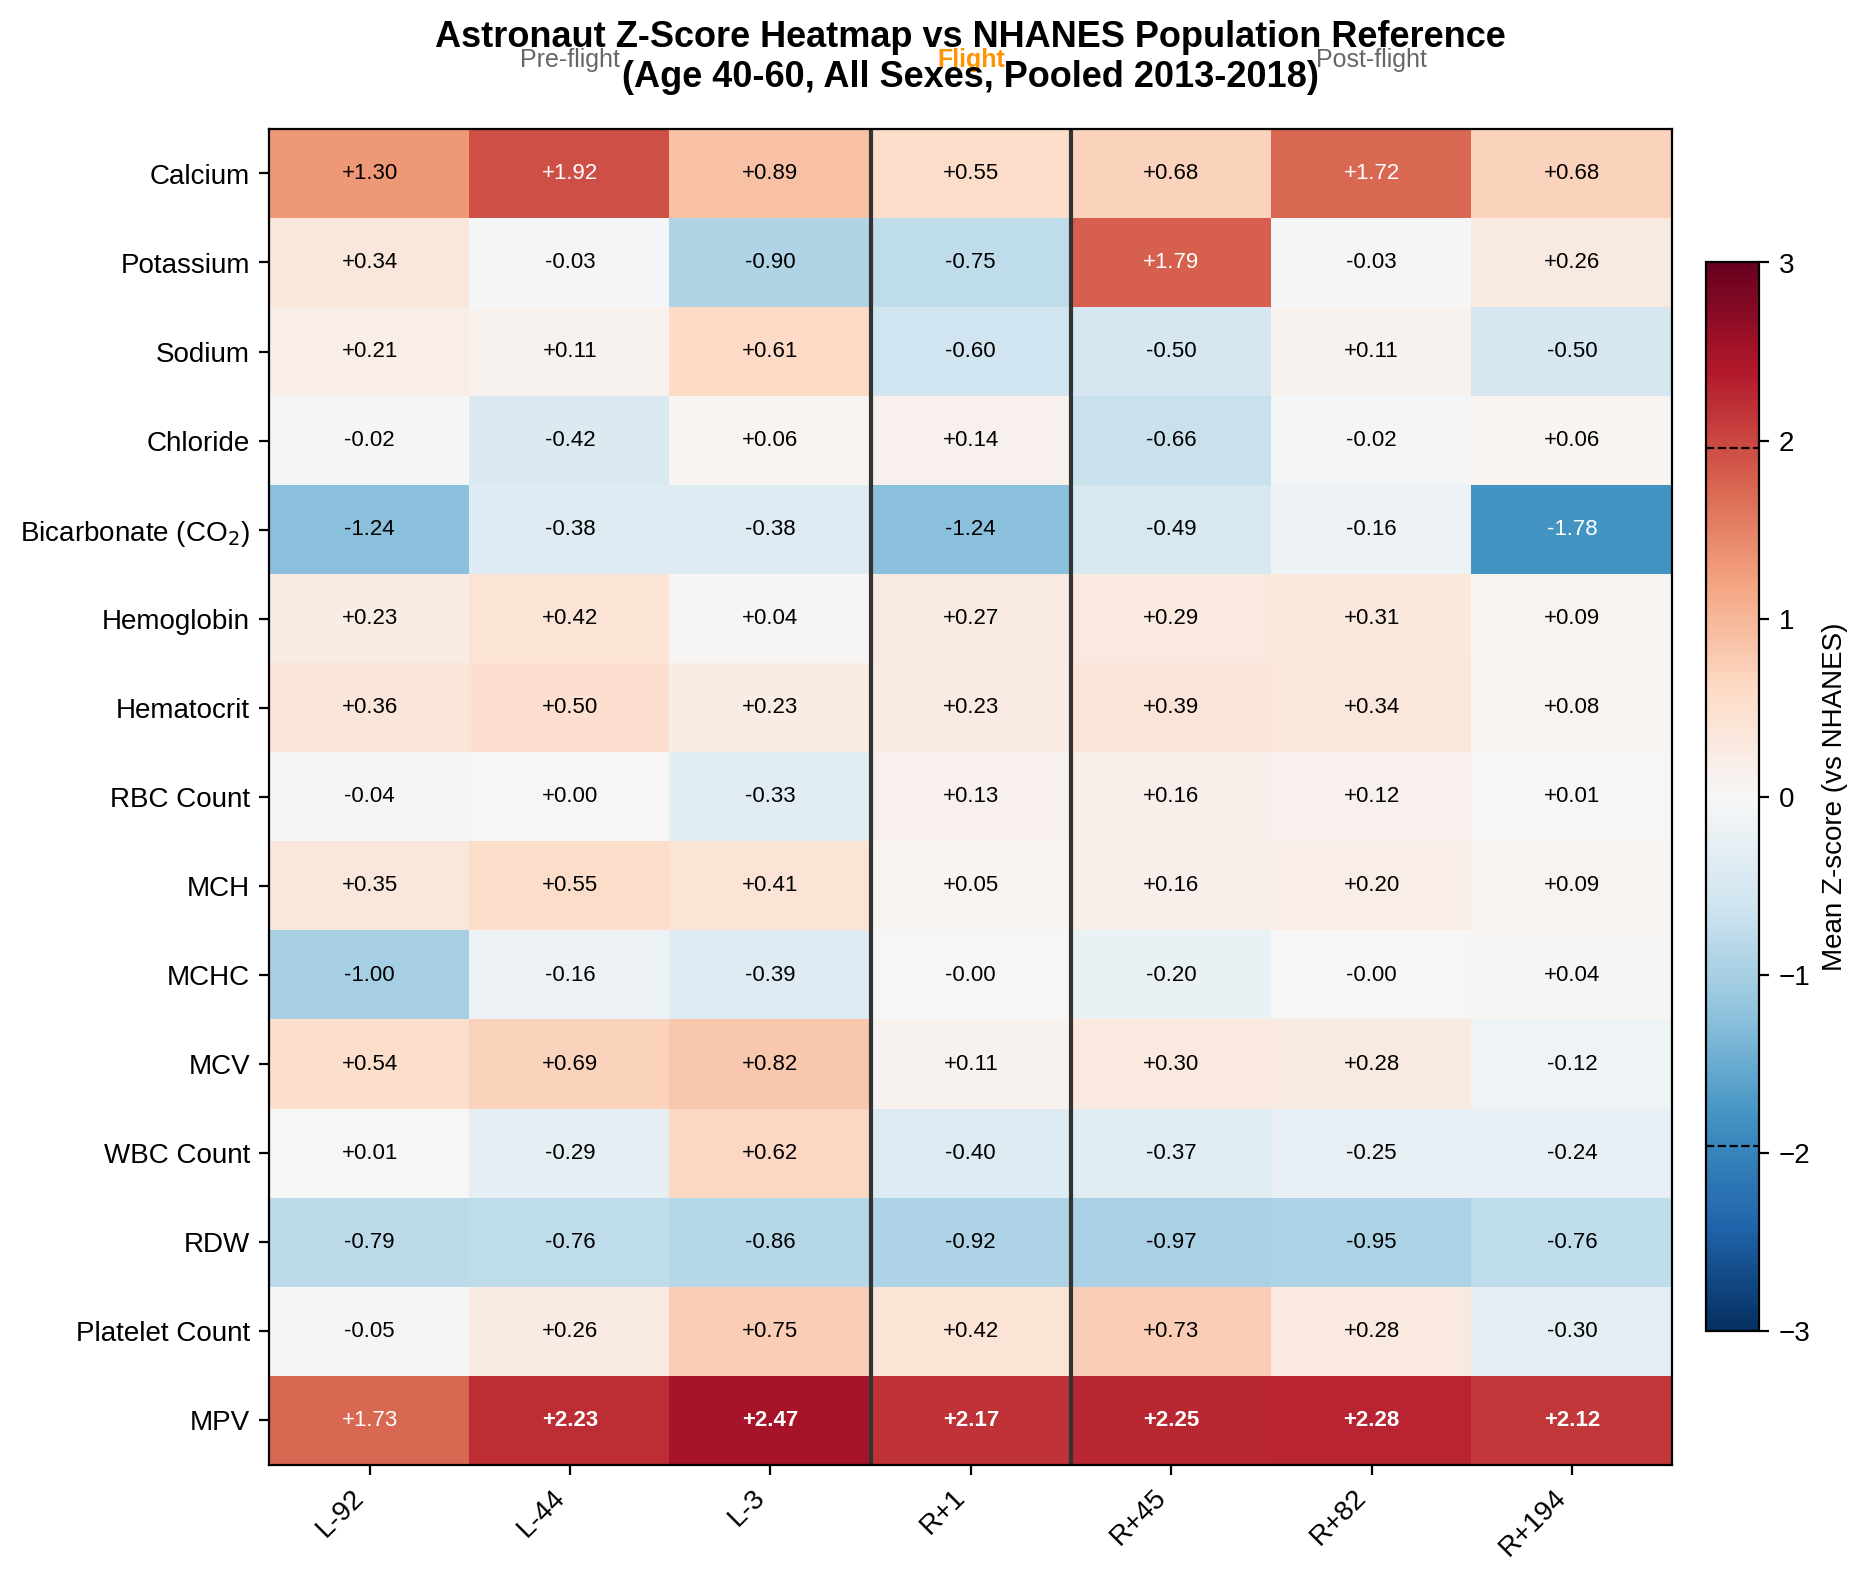
\includegraphics[width=0.85\textwidth]{figures/fig_s7_zscore_heatmap.png}
\caption{Astronaut z-score heatmap against NHANES population reference (age 40--60, all sexes, pooled 2013--2018). Cell values represent mean astronaut z-scores for each variable at each timepoint. Bold text indicates $|z| \geq 1.96$ (population-significant deviation). Diverging colormap centered at zero (blue = below population mean, red = above). Vertical lines separate pre-flight (L-92, L-44, L-3), flight (R+1), and post-flight (R+45, R+82, R+194) phases.}
\label{fig:zscore_heatmap}
\end{figure}

Calcium showed large positive effect sizes at multiple timepoints (Cohen's $d = 1.30$ at L-92, $d = 1.92$ at L-44, $d = 1.72$ at R+82), with 17.9\% of measurements outside the reference interval. Notably, calcium z-scores were elevated even at pre-flight baseline (L-92: $d = 1.30$; L-44: $d = 1.92$), indicating that this population deviation pre-dates spaceflight exposure. Bicarbonate (CO$_2$) was consistently below the population mean ($d = -1.24$ at L-92 and R+1; $d = -1.78$ at R+194), with 14.3\% of measurements outside the lower reference bound. RDW was consistently below the population mean ($d = -0.86$ to $-0.97$), with 18.5\% of measurements outside the lower reference bound.

In contrast, sodium, chloride, MCH, MCV, and WBC count remained within the population reference range across all timepoints (0\% outside P2.5--P97.5), indicating these electrolytes and erythrocyte indices are robust to spaceflight-related perturbation at the group level. Hemoglobin, hematocrit, and RBC count showed modest deviations (3.7--7.4\% outside reference) with small effect sizes, consistent with the known mild spaceflight-associated anemia pattern\textsuperscript{6}.

\begin{figure}[H]
\centering
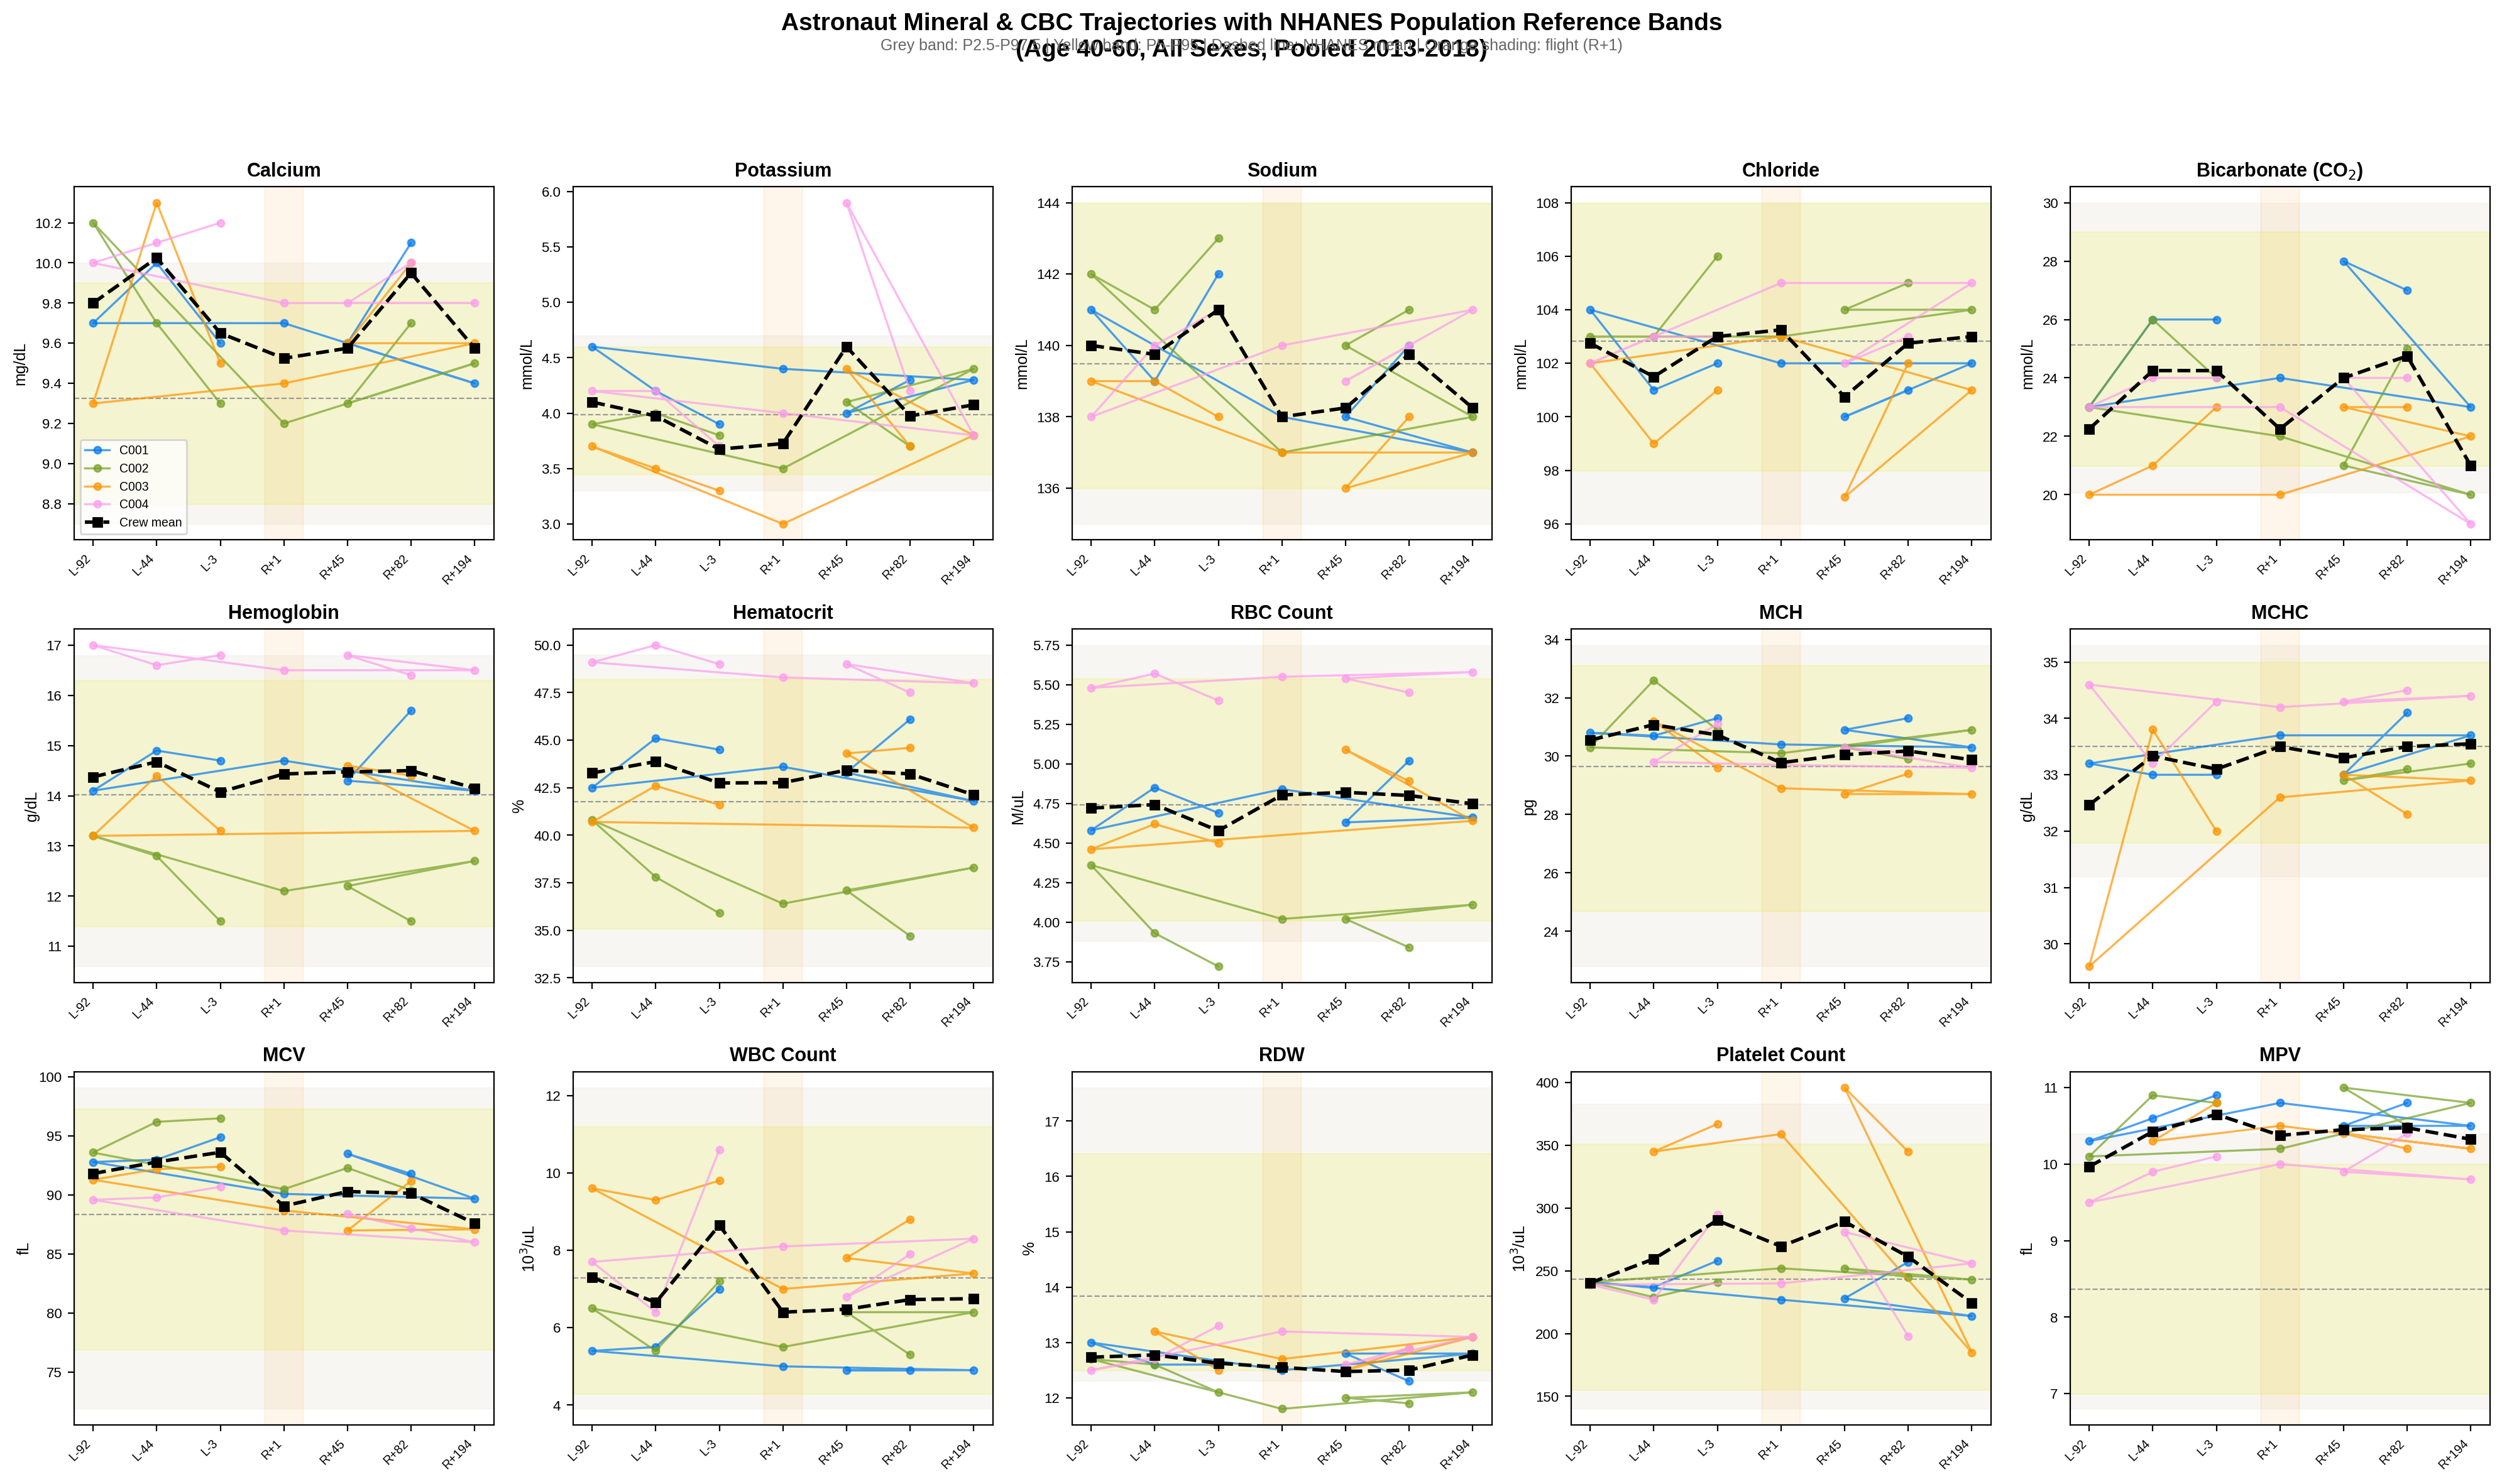
\includegraphics[width=\textwidth]{figures/fig_s6_nhanes_trajectories.png}
\caption{Astronaut mineral and CBC trajectories with NHANES population reference bands. Each panel shows one variable across seven timepoints (L-92 through R+194). Grey band: NHANES P2.5--P97.5 reference interval; yellow band: P5--P95; dashed line: NHANES mean. Colored lines: four individual astronauts; black squares: crew mean. Orange shading marks the flight timepoint (R+1). Reference population: age 40--60, all sexes, pooled NHANES 2013--2018 ($n = 5{,}748$).}
\label{fig:trajectories}
\end{figure}

The trajectory plots (Figure~\ref{fig:trajectories}) reveal that several population-deviating markers (calcium, MPV, bicarbonate) show deviations at pre-flight baseline, while others (potassium at R+45, $d = 1.79$) show transient spaceflight-associated shifts. Percentile ranks for all measurements are shown in Supplementary Figure~S1, and full one-sample test results are provided in Table~\ref{tab:onesample}.

\begin{table}[H]
\centering
\caption{One-sample test results for astronaut markers with large population deviations. Cohen's $d$ computed using NHANES pooled SD. FDR: Benjamini--Hochberg adjusted $p$-value across 105 tests.}
\label{tab:onesample}
\begin{tabular}{llrrrr}
\toprule
\textbf{Variable} & \textbf{Timepoint} & \textbf{Cohen's $d$} & \textbf{$t$ $p$-value} & \textbf{FDR} & \textbf{\% outside ref} \\
\midrule
\multicolumn{6}{l}{\textit{FDR-significant ($< 0.05$)}} \\
MPV & L-3 & 2.47 & 0.001 & 0.048 & 75.0 \\
MPV & R+82 & 2.28 & 0.0005 & 0.047 & 50.0 \\
MPV & L-44 & 2.23 & 0.002 & 0.048 & 50.0 \\
MPV & R+45 & 2.25 & 0.003 & 0.048 & 50.0 \\
MPV & R+1 & 2.17 & 0.001 & 0.048 & 50.0 \\
MPV & R+194 & 2.12 & 0.003 & 0.048 & 50.0 \\
\midrule
\multicolumn{6}{l}{\textit{Large effect ($|d| \geq 0.8$), not FDR-significant}} \\
Calcium & L-44 & 1.92 & 0.011 & 0.115 & 50.0 \\
Potassium & R+45 & 1.79 & 0.257 & 0.649 & 25.0 \\
Bicarbonate & R+194 & $-1.78$ & 0.020 & 0.135 & 25.0 \\
MPV & L-92 & 1.73 & 0.022 & 0.135 & 50.0 \\
Calcium & R+82 & 1.72 & 0.006 & 0.065 & 25.0 \\
Calcium & L-92 & 1.30 & 0.095 & 0.358 & 25.0 \\
Bicarbonate & L-92 & $-1.24$ & 0.031 & 0.164 & 25.0 \\
Bicarbonate & R+1 & $-1.24$ & 0.043 & 0.202 & 25.0 \\
MCHC & L-92 & $-1.00$ & 0.558 & 0.877 & 0.0 \\
RDW & R+45 & $-0.97$ & 0.004 & 0.061 & 0.0 \\
RDW & R+82 & $-0.95$ & 0.012 & 0.115 & 0.0 \\
RDW & R+1 & $-0.92$ & 0.021 & 0.134 & 0.0 \\
Potassium & L-3 & $-0.90$ & 0.100 & 0.363 & 0.0 \\
Calcium & L-3 & 0.89 & 0.194 & 0.599 & 25.0 \\
RDW & L-3 & $-0.86$ & 0.017 & 0.134 & 0.0 \\
MCV & L-3 & 0.82 & 0.027 & 0.156 & 0.0 \\
\bottomrule
\end{tabular}
\end{table}

\subsection{Mineral-pathway transcriptomic response to spaceflight}

To connect the population-deviating clinical markers to molecular mechanisms, we constructed curated mineral homeostasis gene sets for 10 minerals (calcium, iron, magnesium, zinc, copper, selenium, potassium, sodium, phosphorus, manganese) from KEGG pathways and published literature, yielding 801 unique genes. Five KEGG pathways relevant to mineral metabolism were included: mineral absorption (hsa04978, 61 genes), calcium signaling (hsa04020, 254 genes), ferroptosis (hsa04216, 42 genes), oxidative phosphorylation (hsa00190, 138 genes), and bile secretion (hsa04976, 90 genes). Of these, 784 genes were mapped to the astronaut RNA-seq feature space.

Differential expression analysis across three flight comparisons (I4-FP1: R+1 vs.\ pre-flight; I4-FP2: R+1/R+45/R+82 vs.\ pre-flight; I4-FP3: all post-flight vs.\ pre-flight) identified 50 unique mineral-pathway genes with $|\log_2\text{FC}| > 0.5$ and $p < 0.05$ (71 total entries across omics layers and comparisons; Figure~\ref{fig:de_heatmap}).

\begin{figure}[H]
\centering
\begin{subfigure}{0.55\textwidth}
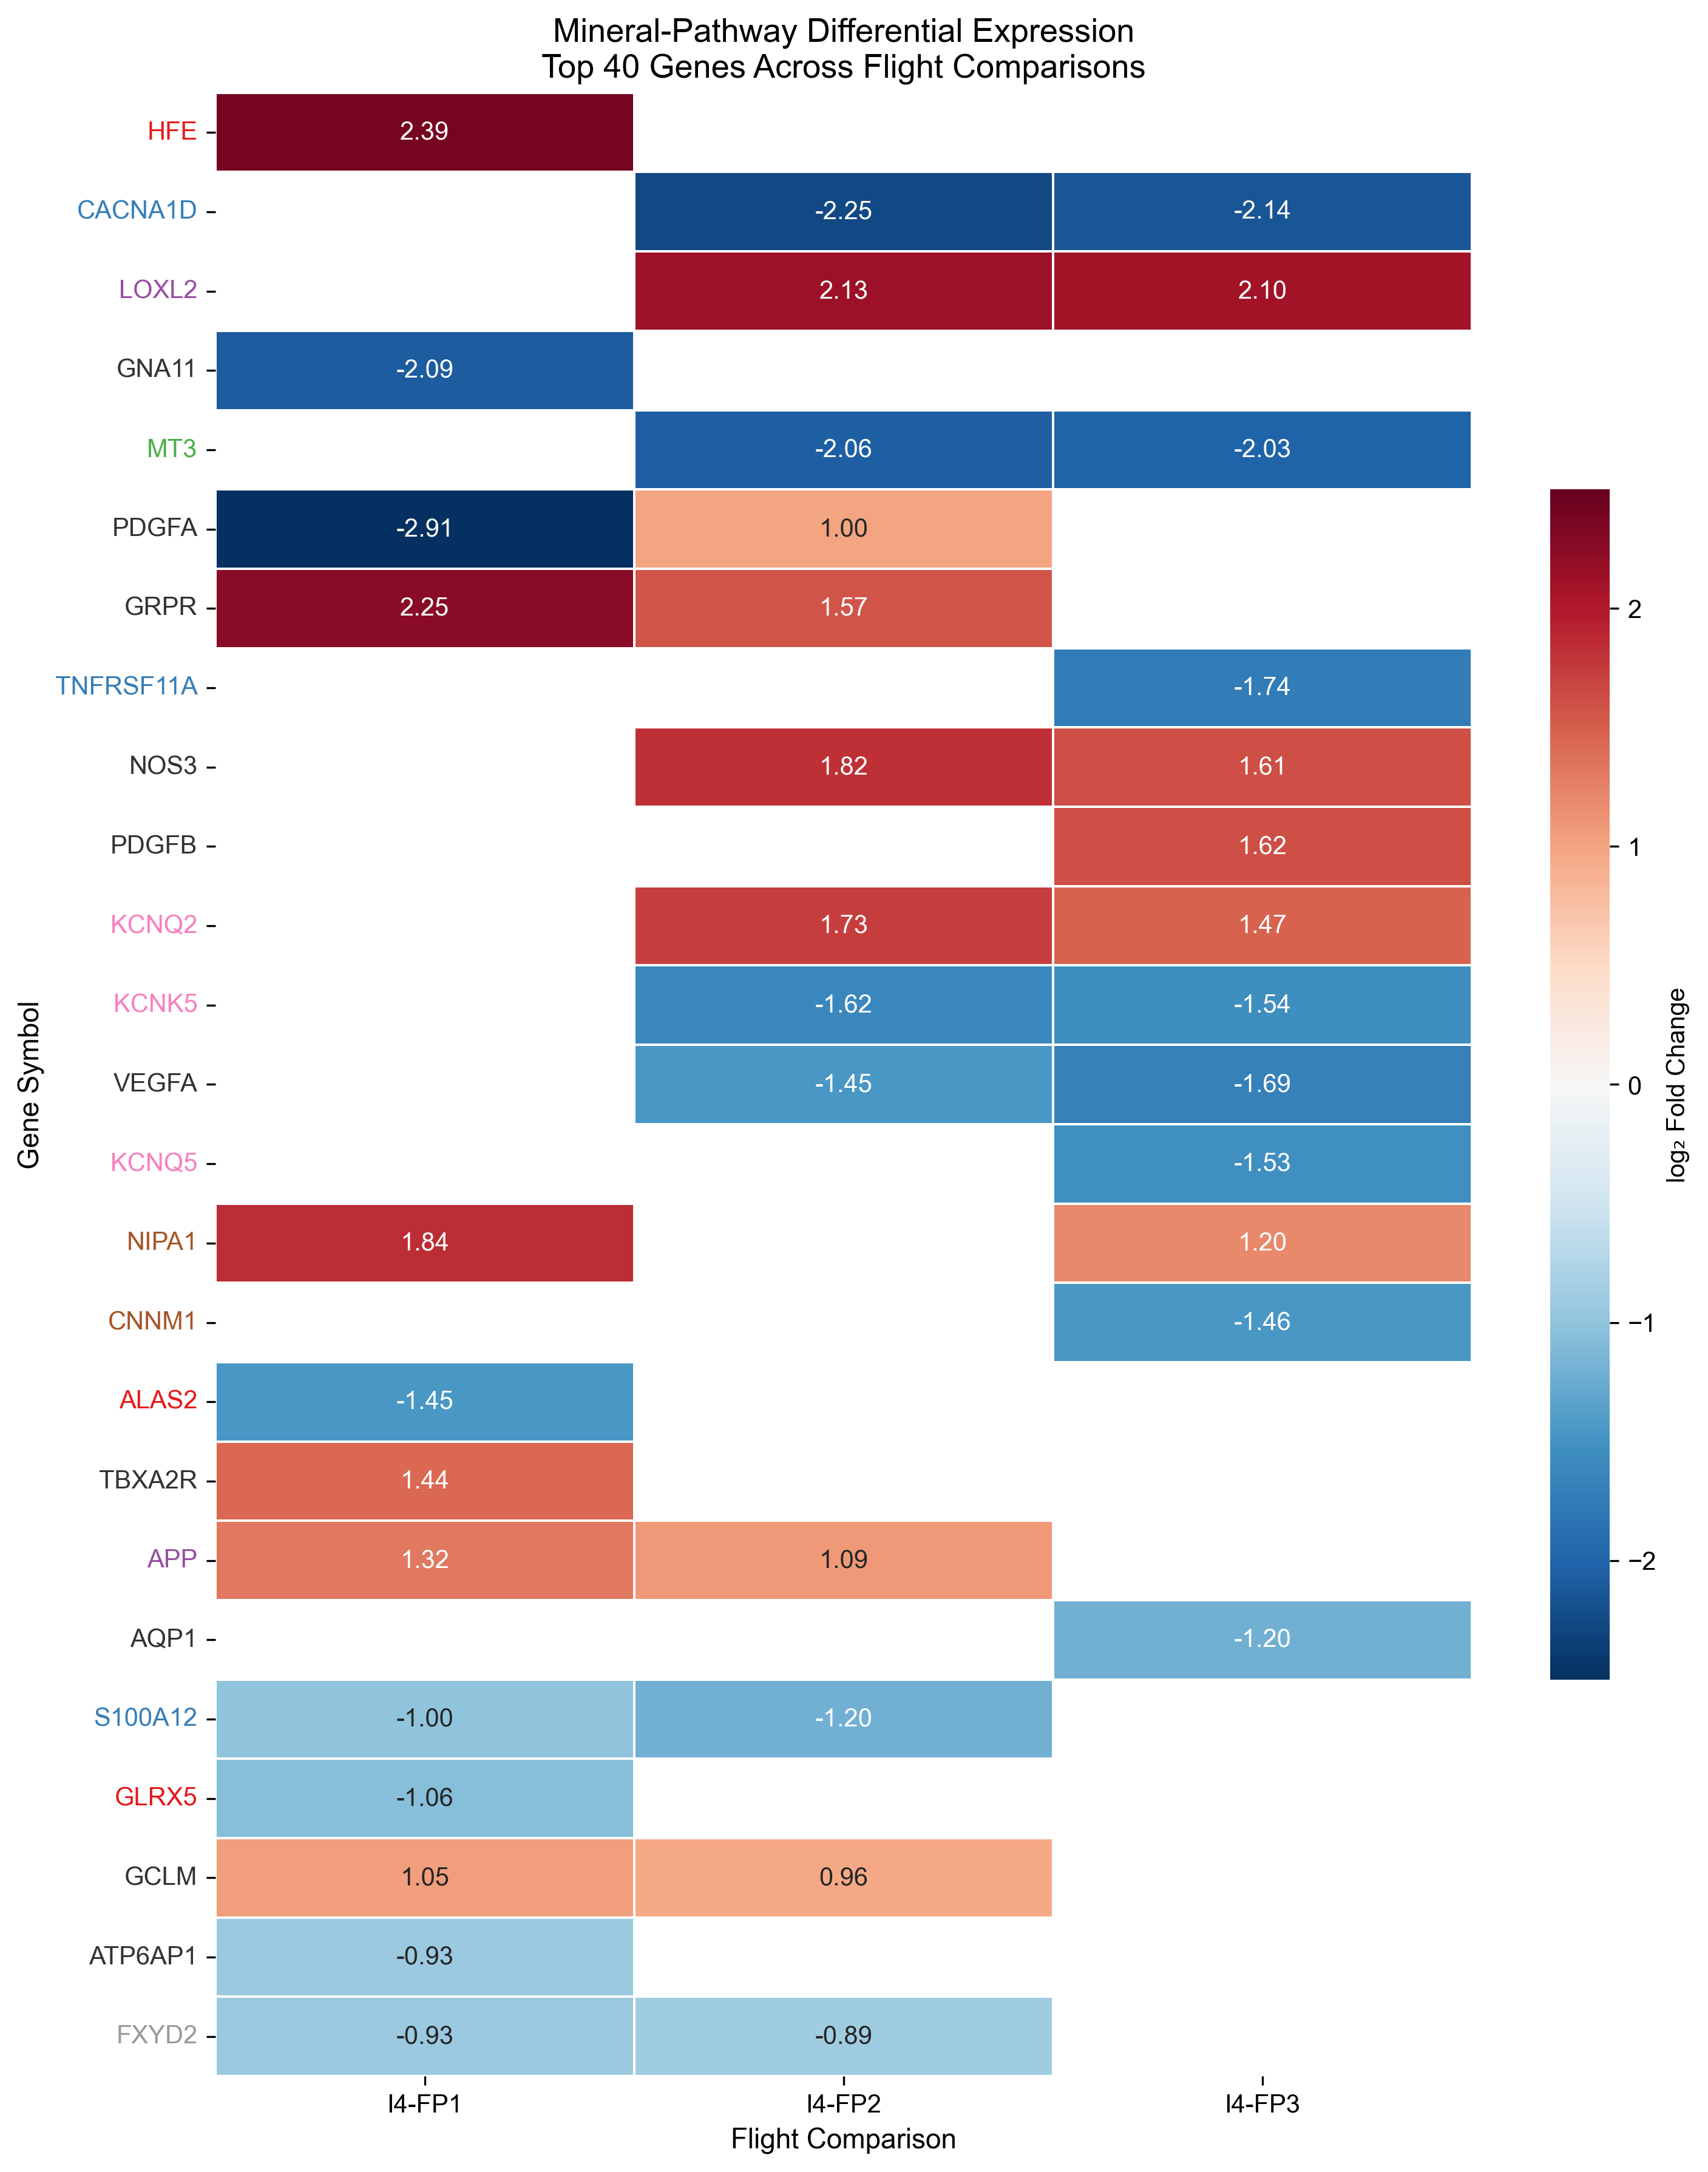
\includegraphics[width=\textwidth]{figures/fig1_heatmap_mineral_de.png}
\caption{}
\end{subfigure}
\hfill
\begin{subfigure}{0.43\textwidth}
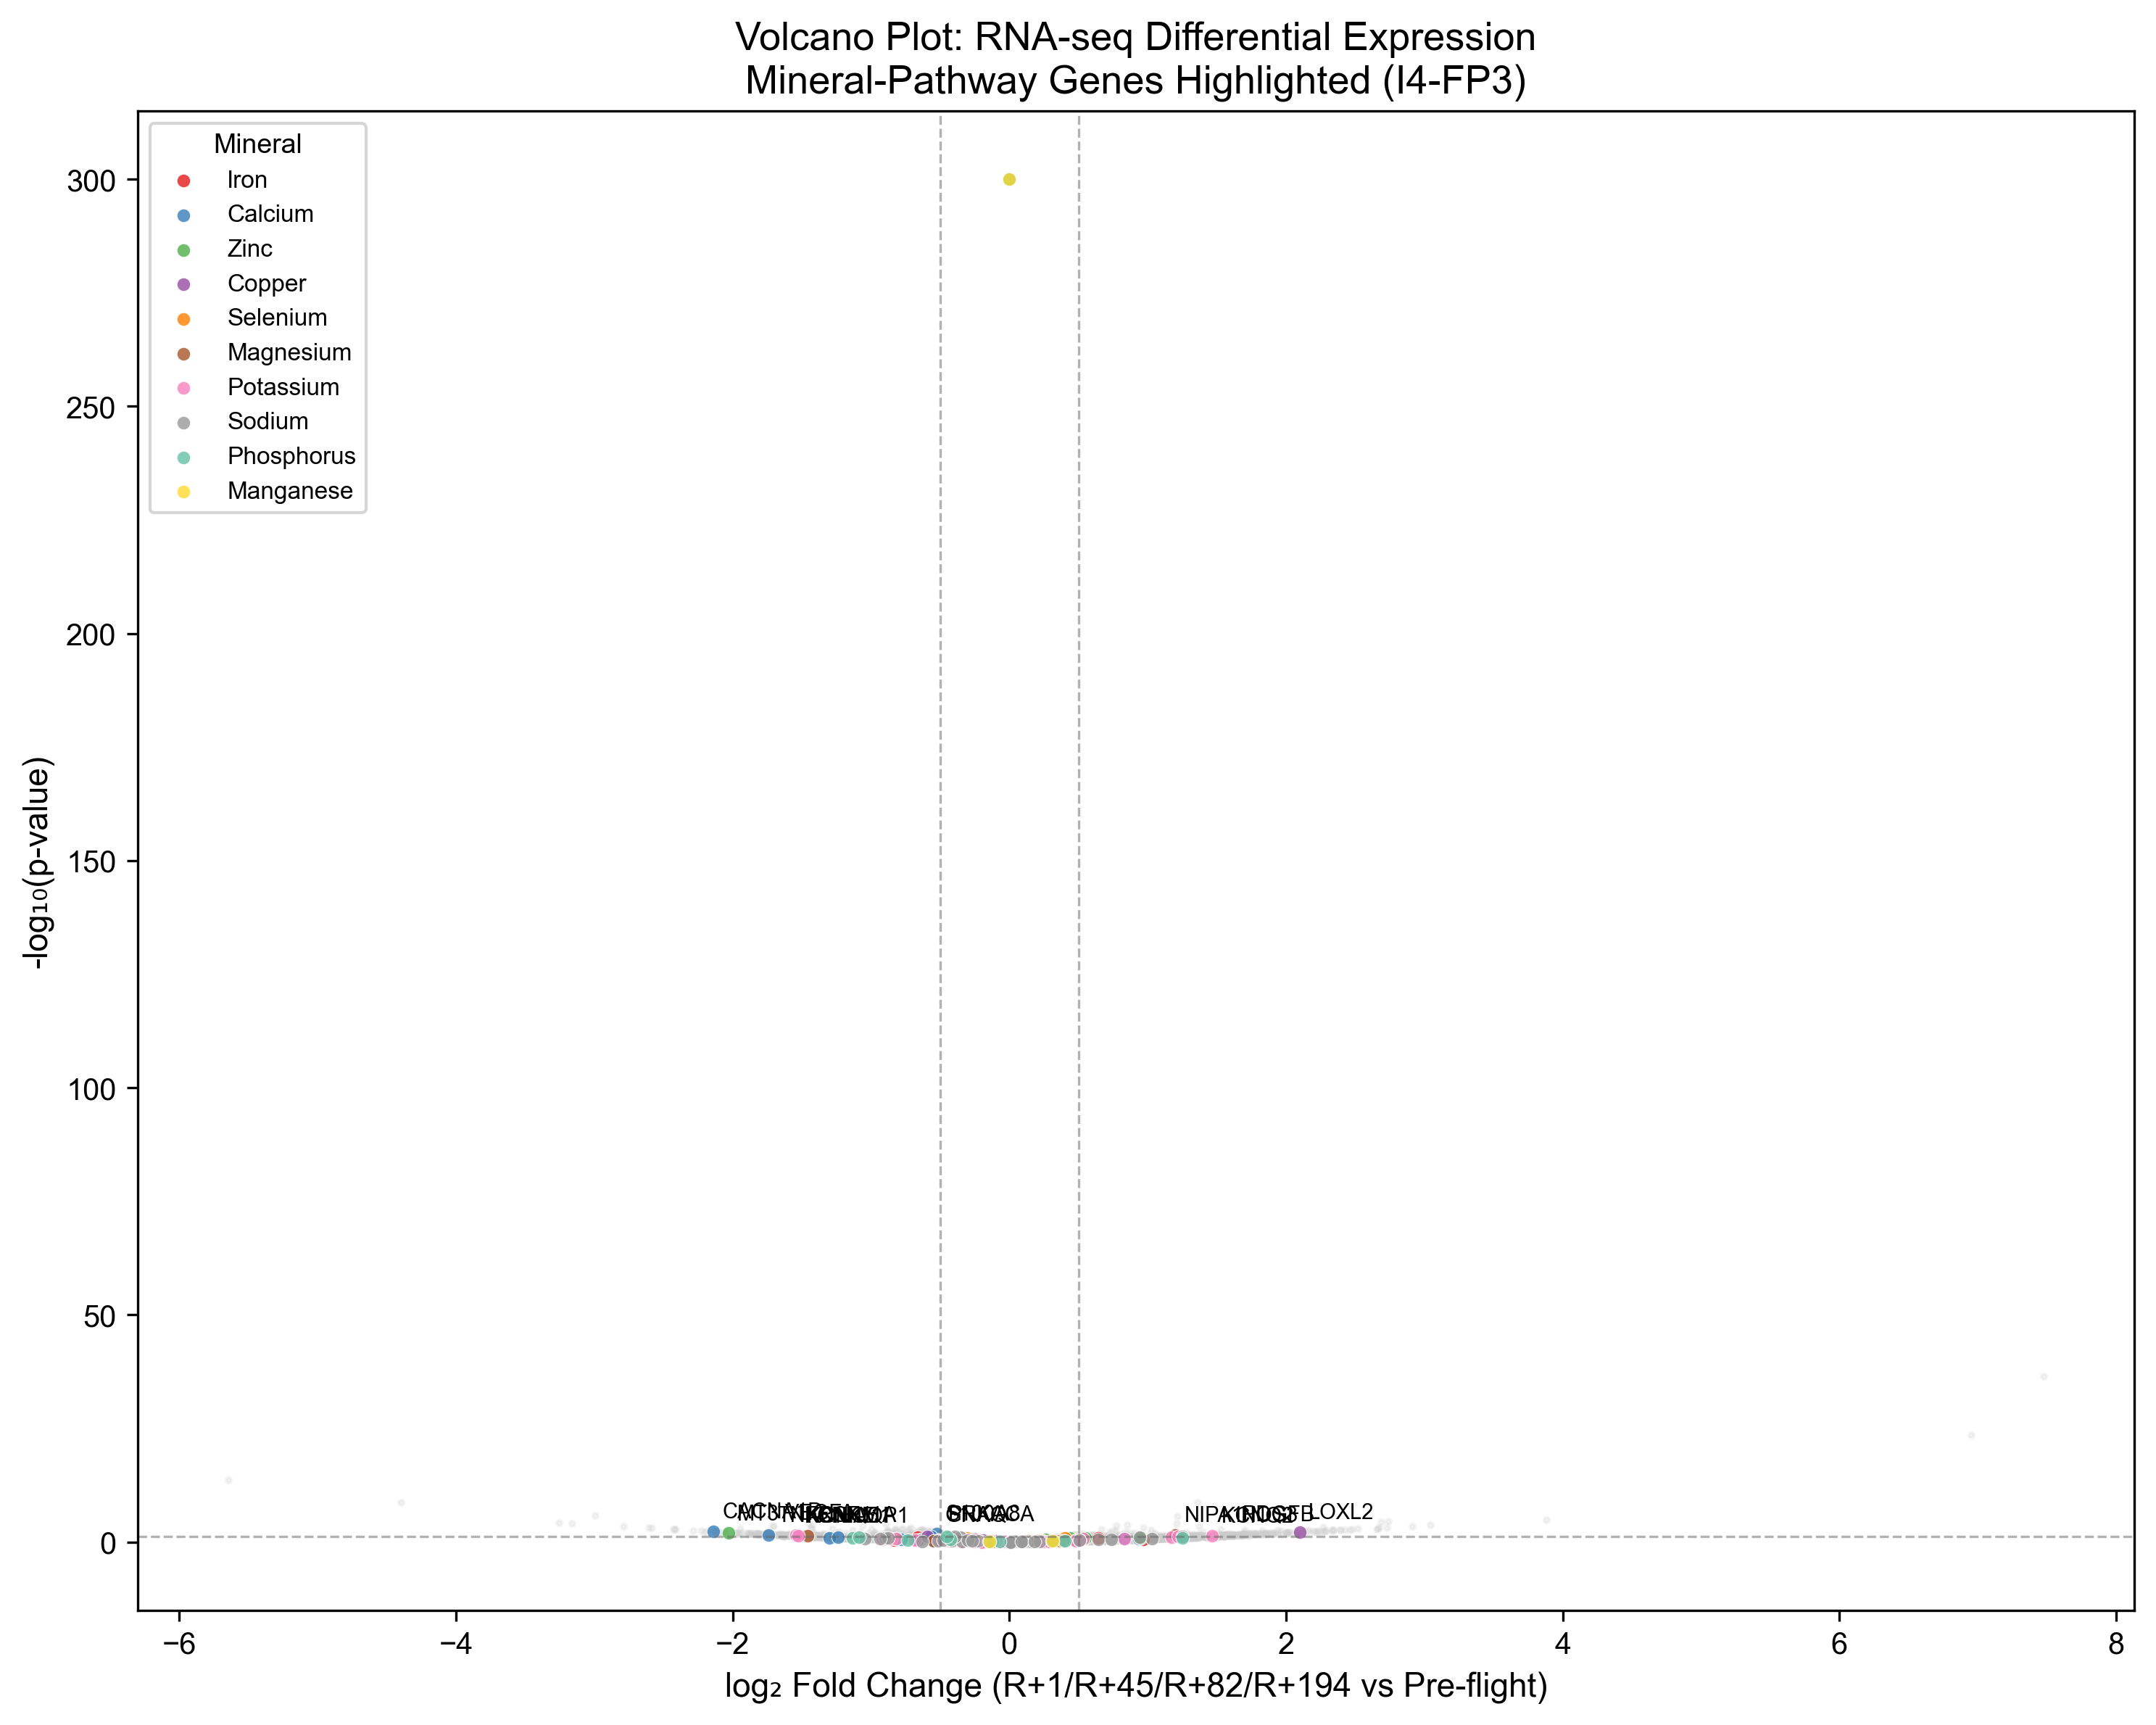
\includegraphics[width=\textwidth]{figures/fig2_volcano_rnaseq.png}
\caption{}
\end{subfigure}
\caption{Mineral-pathway differential expression. (a) Heatmap of significant mineral-pathway DE genes ($|\log_2\text{FC}| > 0.5$, $p < 0.05$) across RNA-seq and proteomics comparisons. Gene annotations indicate primary mineral associations. (b) Volcano plot of RNA-seq differential expression (I4-FP1: R+1 vs.\ pre-flight), with mineral-pathway genes highlighted by mineral association.}
\label{fig:de_heatmap}
\end{figure}

The most consistent findings were: \textbf{Copper pathway} --- APP (amyloid precursor protein, copper-binding) was up-regulated in proteomics ($\log_2\text{FC} = 1.32$, FDR $= 0.001$), while LOX and LOXL1 (copper-dependent lysyl oxidases) were down-regulated. LOXL2 was up-regulated in RNA-seq ($\log_2\text{FC} = 2.10$). Lysyl oxidases are critical for collagen cross-linking and connective tissue integrity\textsuperscript{7}. \textbf{Iron pathway} --- ALAS2 (erythroid-specific aminolevulinate synthase) was down-regulated ($\log_2\text{FC} = -1.45$, FDR $= 0.008$), while HFE (hemochromatosis gene) was up-regulated ($\log_2\text{FC} = 2.39$). GLRX5 was also down-regulated. These changes are consistent with the space-flight anemia and increased iron availability reported in astronauts\textsuperscript{6}. \textbf{Magnesium pathway} --- NIPA1 was up-regulated ($\log_2\text{FC} = 1.84$). \textbf{Calcium pathway} --- S100A8, S100A9, and S100A12 (calcium-binding calgranulins) were down-regulated in proteomics and RNA-seq; S100A8/A9 form calprotectin, a key innate immune mediator\textsuperscript{8}. CACNA1D (voltage-gated calcium channel) showed the largest fold change ($\log_2\text{FC} = -2.25$ in I4-FP2, $-2.14$ in I4-FP3), potentially reflecting cellular adaptation to mechanical unloading, which alters mechanotransduction signalling\textsuperscript{9}. \textbf{Zinc pathway} --- MT2A and MT3 (metallothioneins) were down-regulated ($\log_2\text{FC} = -0.75$ to $-2.03$). \textbf{Potassium pathway} --- KCNQ2 was up-regulated ($\log_2\text{FC} = 1.73$), while FXYD2 (sodium/potassium transport regulator) was down-regulated in proteomics.

Gene set enrichment analysis (GSEA) revealed down-regulation of oxidative phosphorylation (NES $= -1.63$, NOM $p = 0.002$) and the iron mineral gene set (NES $= -1.53$, NOM $p = 0.037$) in the I4-FP1 comparison, while ferroptosis showed a trend toward up-regulation (NES $= 1.37$, NOM $p = 0.052$; Supplementary Figure~S2). Time-resolved pathway activation patterns are shown in Supplementary Figure~S3.

\subsection{Machine learning: mineral-pathway genes predict serum mineral levels}

We evaluated whether mineral-pathway gene expression carries predictive information about serum mineral levels using two complementary machine learning approaches.

\subsubsection{Regression analysis (mineral level prediction)}

Four regressors (Ridge, SVR-Linear, SVR-RBF, RandomForest) were trained to predict serum calcium, potassium, sodium, and hemoglobin (iron proxy) from mineral-pathway gene expression under leave-one-out cross-validation (LOO-CV, $n = 16$). The top 200 genes by variance were used as features. Potassium was predicted with $r = 0.50$ ($R^2 = 0.12$, Ridge regression) and sodium with $r = 0.46$ ($R^2 = 0.19$, SVR-Linear). Hemoglobin was predicted with $r = 0.48$ (SVR-Linear), though the negative $R^2$ ($-0.62$) indicates the model performs worse than the mean baseline on held-out samples. Calcium showed no predictive signal ($r = -0.02$).

Permutation importance analysis identified \textit{CAMK4} (calcium signaling), \textit{SLC30A7} (zinc transporter), \textit{SELENOW} (selenium protein), \textit{SLC11A1} (iron transporter), and \textit{ALPL} (calcium/phosphorus) as top predictive genes for potassium, and \textit{CAMK4}, \textit{ITPKB}, \textit{SLC2A1}, and \textit{PPP3R1} for sodium (Figure~\ref{fig:ml_results}a). The contribution of genes from multiple mineral pathways to predicting individual minerals highlights the interconnectedness of mineral homeostasis systems.

\subsubsection{Classification analysis (flight vs.\ ground)}

A revised classification analysis addressed three issues in the initial pipeline: data leakage from feature selection outside cross-validation, lack of imbalance handling, and in-sample permutation importance. Class-weighted elastic-net logistic regression with nested LOO-CV was applied to all 784 mineral-pathway genes, with a 500-permutation significance test.

SVM with RBF kernel achieved AUC $= 1.0$ (perfect ranking) with permutation $p < 0.002$. However, the null distribution was non-standard (mean $= 0.121$), because \texttt{class\_weight='balanced'} biases the classifier toward specificity when labels are shuffled, inflating the apparent significance. The elastic-net models showed no discriminative signal (balanced AUC $= 0.06$--$0.35$, all $p > 0.67$), indicating that linear mineral-pathway gene expression cannot reliably separate flight from ground samples with $n = 4$.

Stability selection identified 16 genes selected in $\geq 50\%$ of LOO folds (Figure~\ref{fig:ml_results}b), enriched in iron metabolism (\textit{HFE} 88\%, \textit{SLC11A2} 81\%, \textit{ALAS2} 69\%, \textit{PCBP2} 69\%) and potassium transport (\textit{KCNE1} 94\%). These results are discovery-only and underpowered; the permutation null distribution and confusion matrices are provided in Supplementary Figure~S4.

\begin{figure}[H]
\centering
\begin{subfigure}{0.48\textwidth}
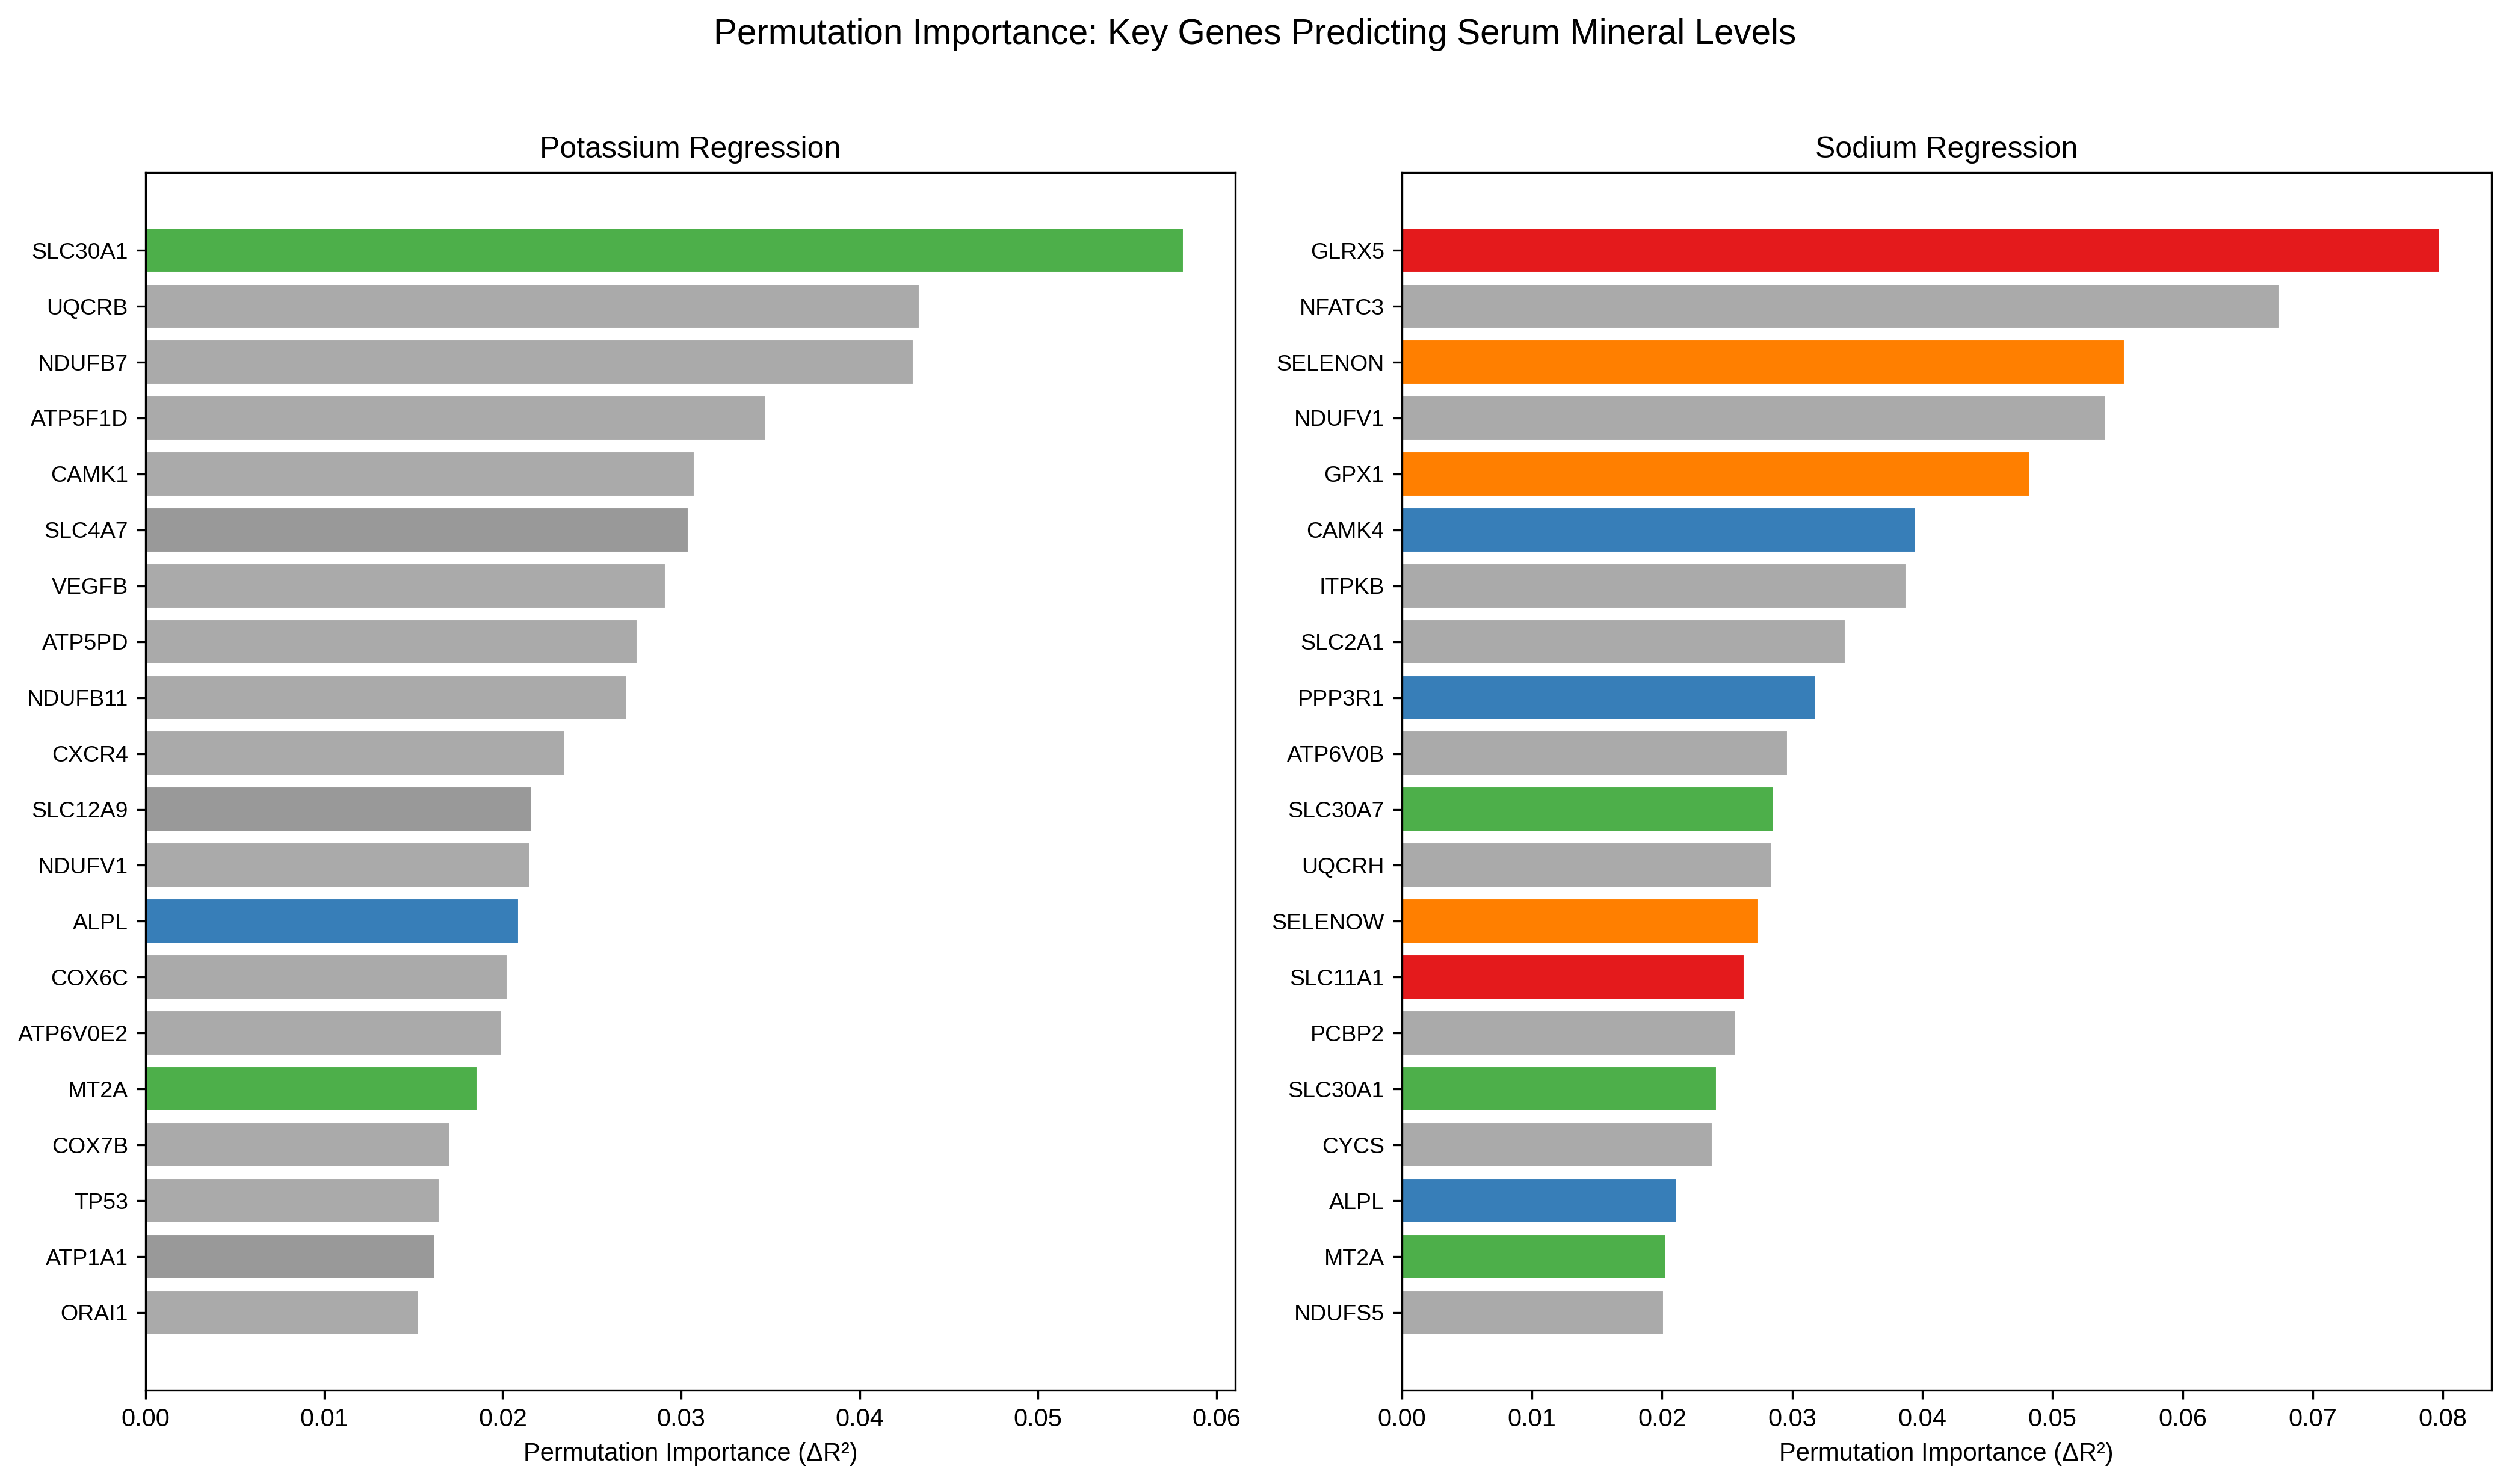
\includegraphics[width=\textwidth]{figures/fig3_barplot_importance.png}
\caption{}
\end{subfigure}
\hfill
\begin{subfigure}{0.48\textwidth}
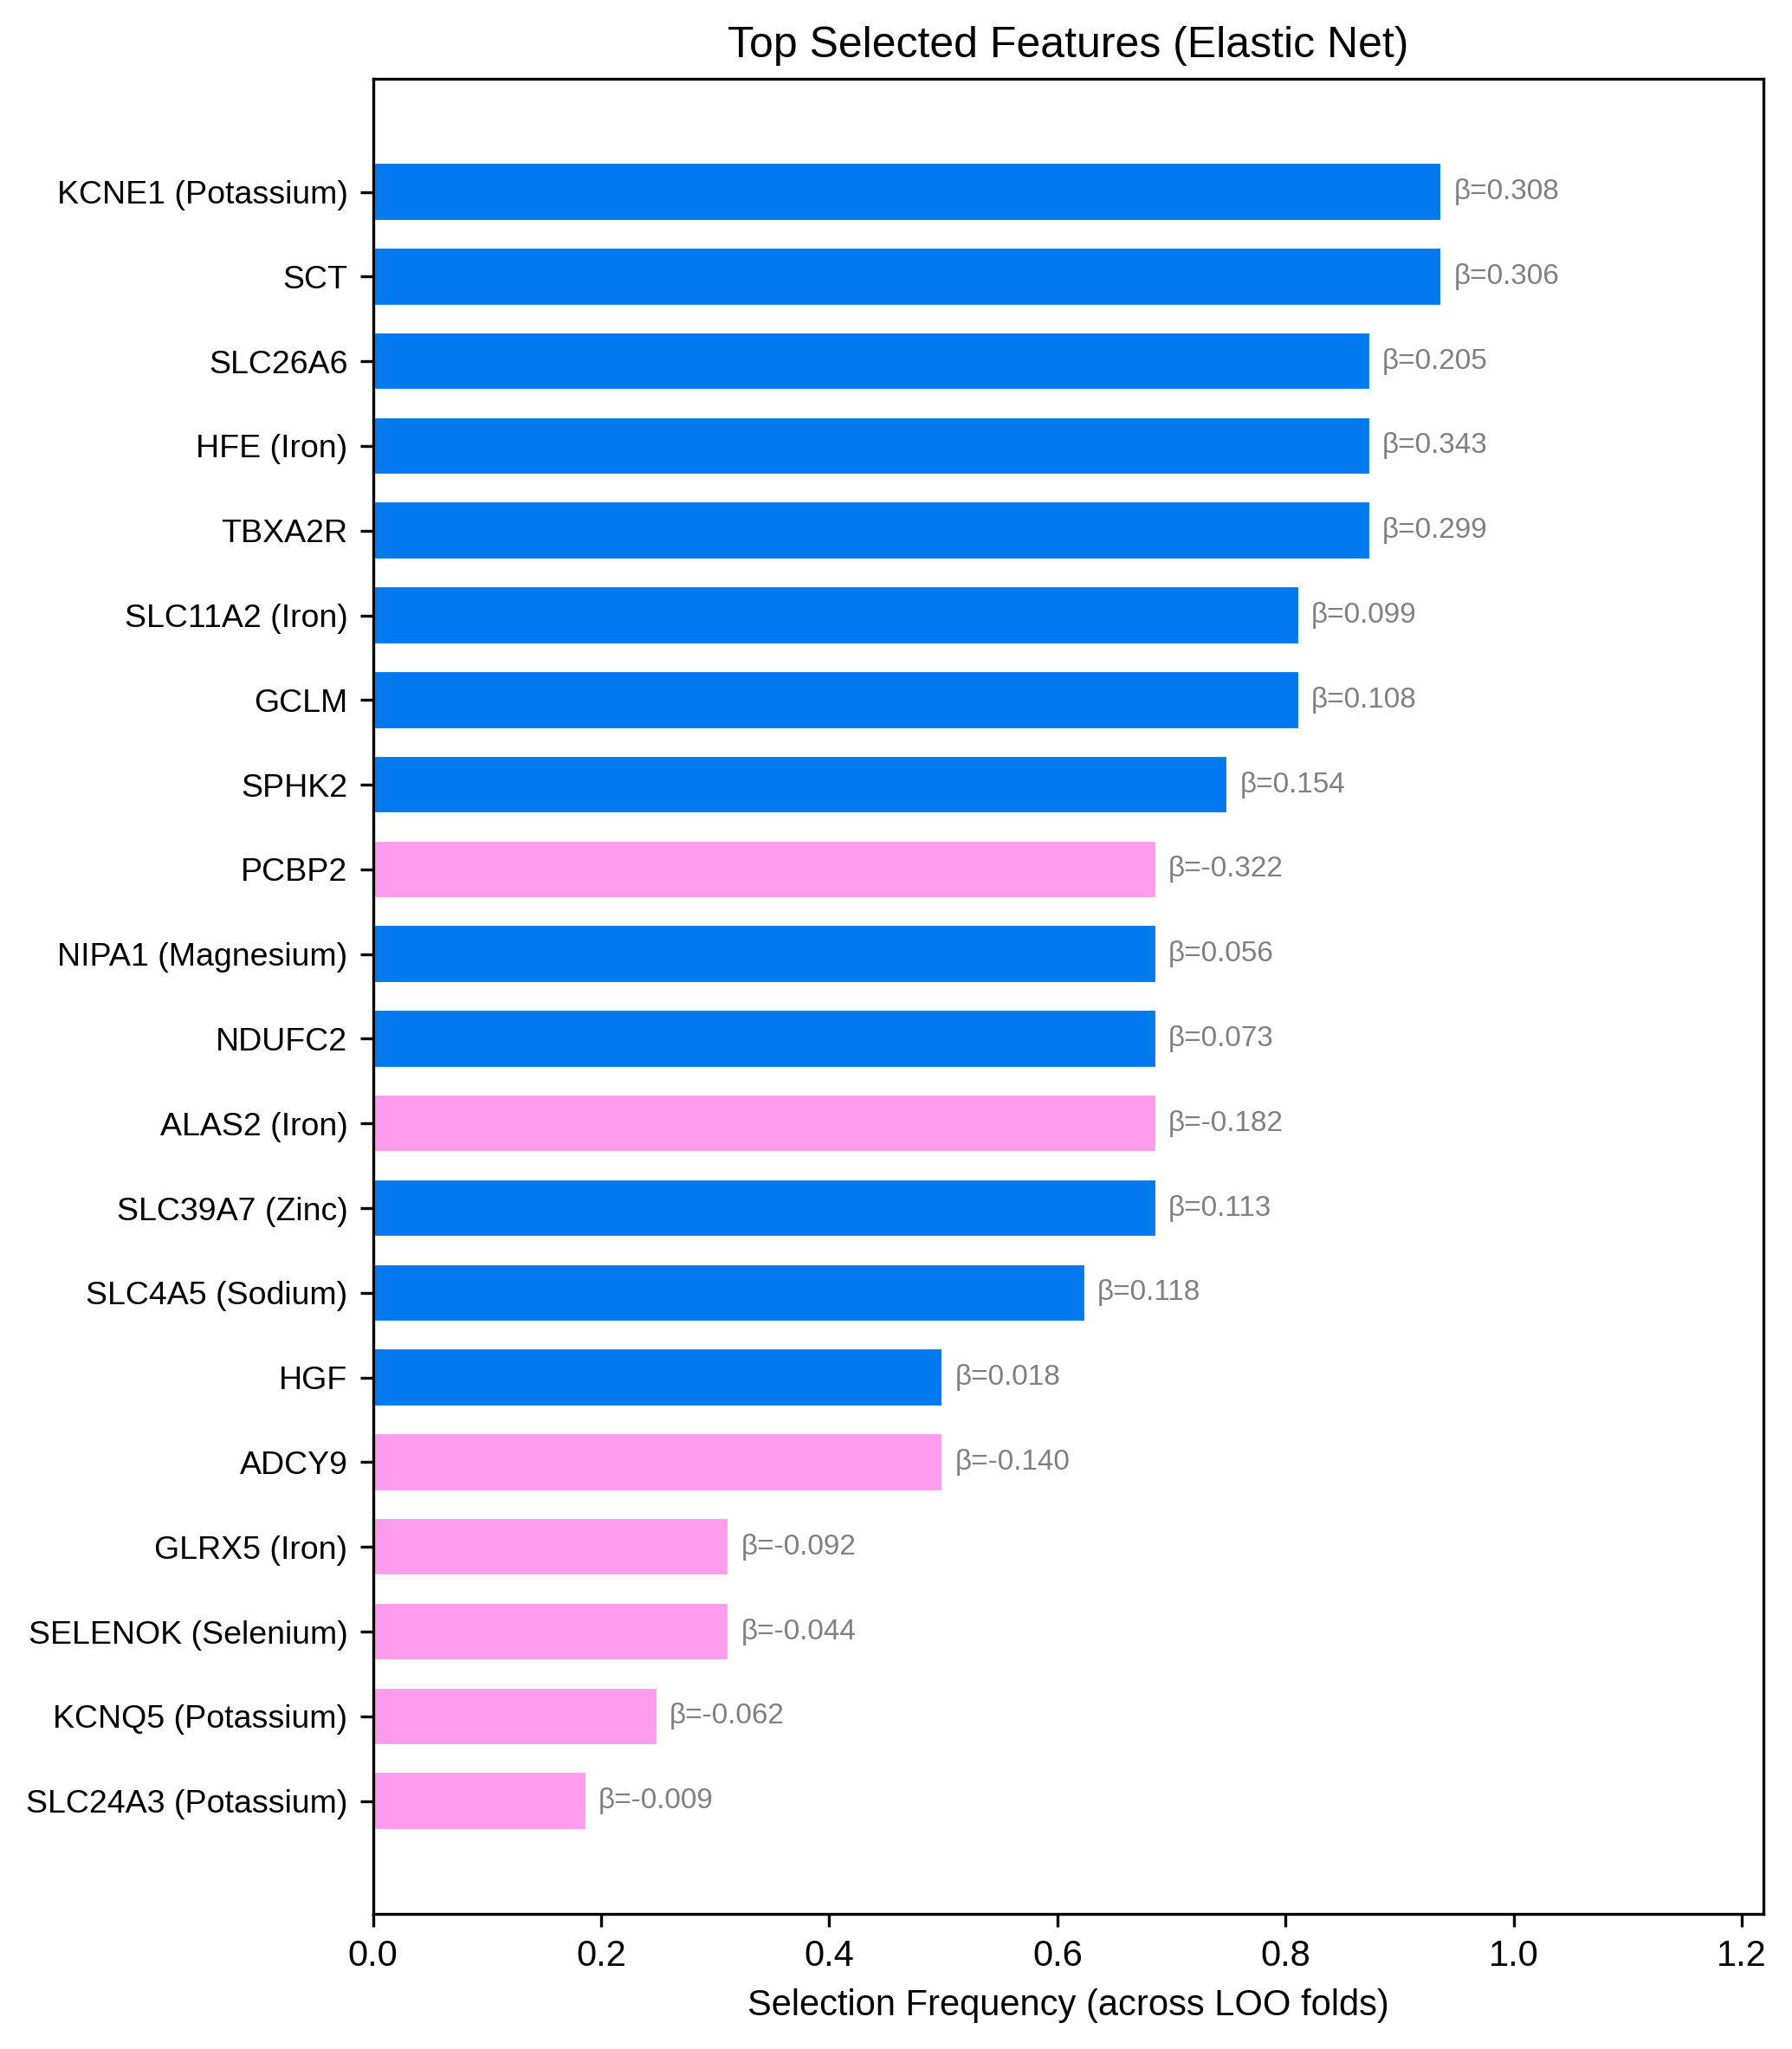
\includegraphics[width=\textwidth]{figures/figS8_selected_features.png}
\caption{}
\end{subfigure}
\caption{Machine learning analysis. (a) Permutation importance for potassium (left) and sodium (right) regression under LOO-CV. Bar colors indicate the primary mineral association of each gene. (b) Stability-selected features from imbalance-aware elastic-net classification: selection frequency across LOO folds and mean coefficient magnitude, annotated with mineral pathway.}
\label{fig:ml_results}
\end{figure}

\begin{table}[H]
\centering
\caption{Machine learning model comparison. Regression (v1): LOO-CV on top-200 variance genes. Classification (v2): nested LOO-CV on 784 mineral-pathway genes with class-weight balancing.}
\label{tab:ml_comparison}
\begin{tabular}{llrr}
\toprule
\textbf{Task} & \textbf{Model} & \textbf{Metric} & \textbf{Value} \\
\midrule
\multicolumn{4}{l}{\textit{Regression (LOO-CV, $n=16$)}} \\
Potassium & Ridge & $r$ / $R^2$ & 0.50 / 0.12 \\
Sodium & SVR-Linear & $r$ / $R^2$ & 0.46 / 0.19 \\
Hemoglobin & SVR-Linear & $r$ / $R^2$ & 0.48 / $-0.62$ \\
Calcium & Ridge & $r$ / $R^2$ & $-0.02$ / $-0.59$ \\
\midrule
\multicolumn{4}{l}{\textit{Classification (nested LOO-CV, 4 flight vs 12 ground)}} \\
SVM-RBF (balanced) & --- & AUC & 1.0 (null mean 0.121, $p < 0.002$) \\
ElasticNet (balanced) & --- & AUC & 0.10 ($p = 0.68$) \\
ElasticNet (filtered) & --- & AUC & 0.35 ($p = 0.68$) \\
Dummy (stratified) & --- & AUC & 0.50 \\
\bottomrule
\end{tabular}
\end{table}

\subsection{Cross-species meta-analysis: muscle-specific concordance}

To assess whether mineral-pathway transcriptional responses are conserved across species, we conducted a Fisher $z$ random-effects meta-analysis across 28 rodent spaceflight datasets from the NASA OSDR, comprising 10 liver, 12 muscle (6 subtypes: EDL, gastrocnemius, quadriceps, soleus, tibialis anterior), and 6 kidney datasets. For each dataset, flight vs.\ ground control differential expression was computed, mapped to human orthologs, and correlated with astronaut peripheral blood mineral-pathway log$_2$FC values.

Skeletal muscle showed significant pooled concordance with astronaut mineral-pathway responses ($r = 0.035$, 95\% CI: 0.012--0.058, $p = 0.0025$; Figure~\ref{fig:cross_species}). The soleus muscle, a postural muscle particularly sensitive to microgravity unloading\textsuperscript{10}, showed the strongest tissue-specific concordance ($r = 0.059$, 95\% CI: 0.015--0.104, $p = 0.009$). Liver ($r = -0.010$, $p = 0.50$) and kidney ($r = -0.016$, $p = 0.40$) showed no significant concordance. Across all 28 datasets combined, the pooled effect was not significant ($r = 0.008$, $p = 0.41$), with moderate heterogeneity ($I^2 = 31\%$).

\begin{figure}[H]
\centering
\begin{subfigure}{0.55\textwidth}
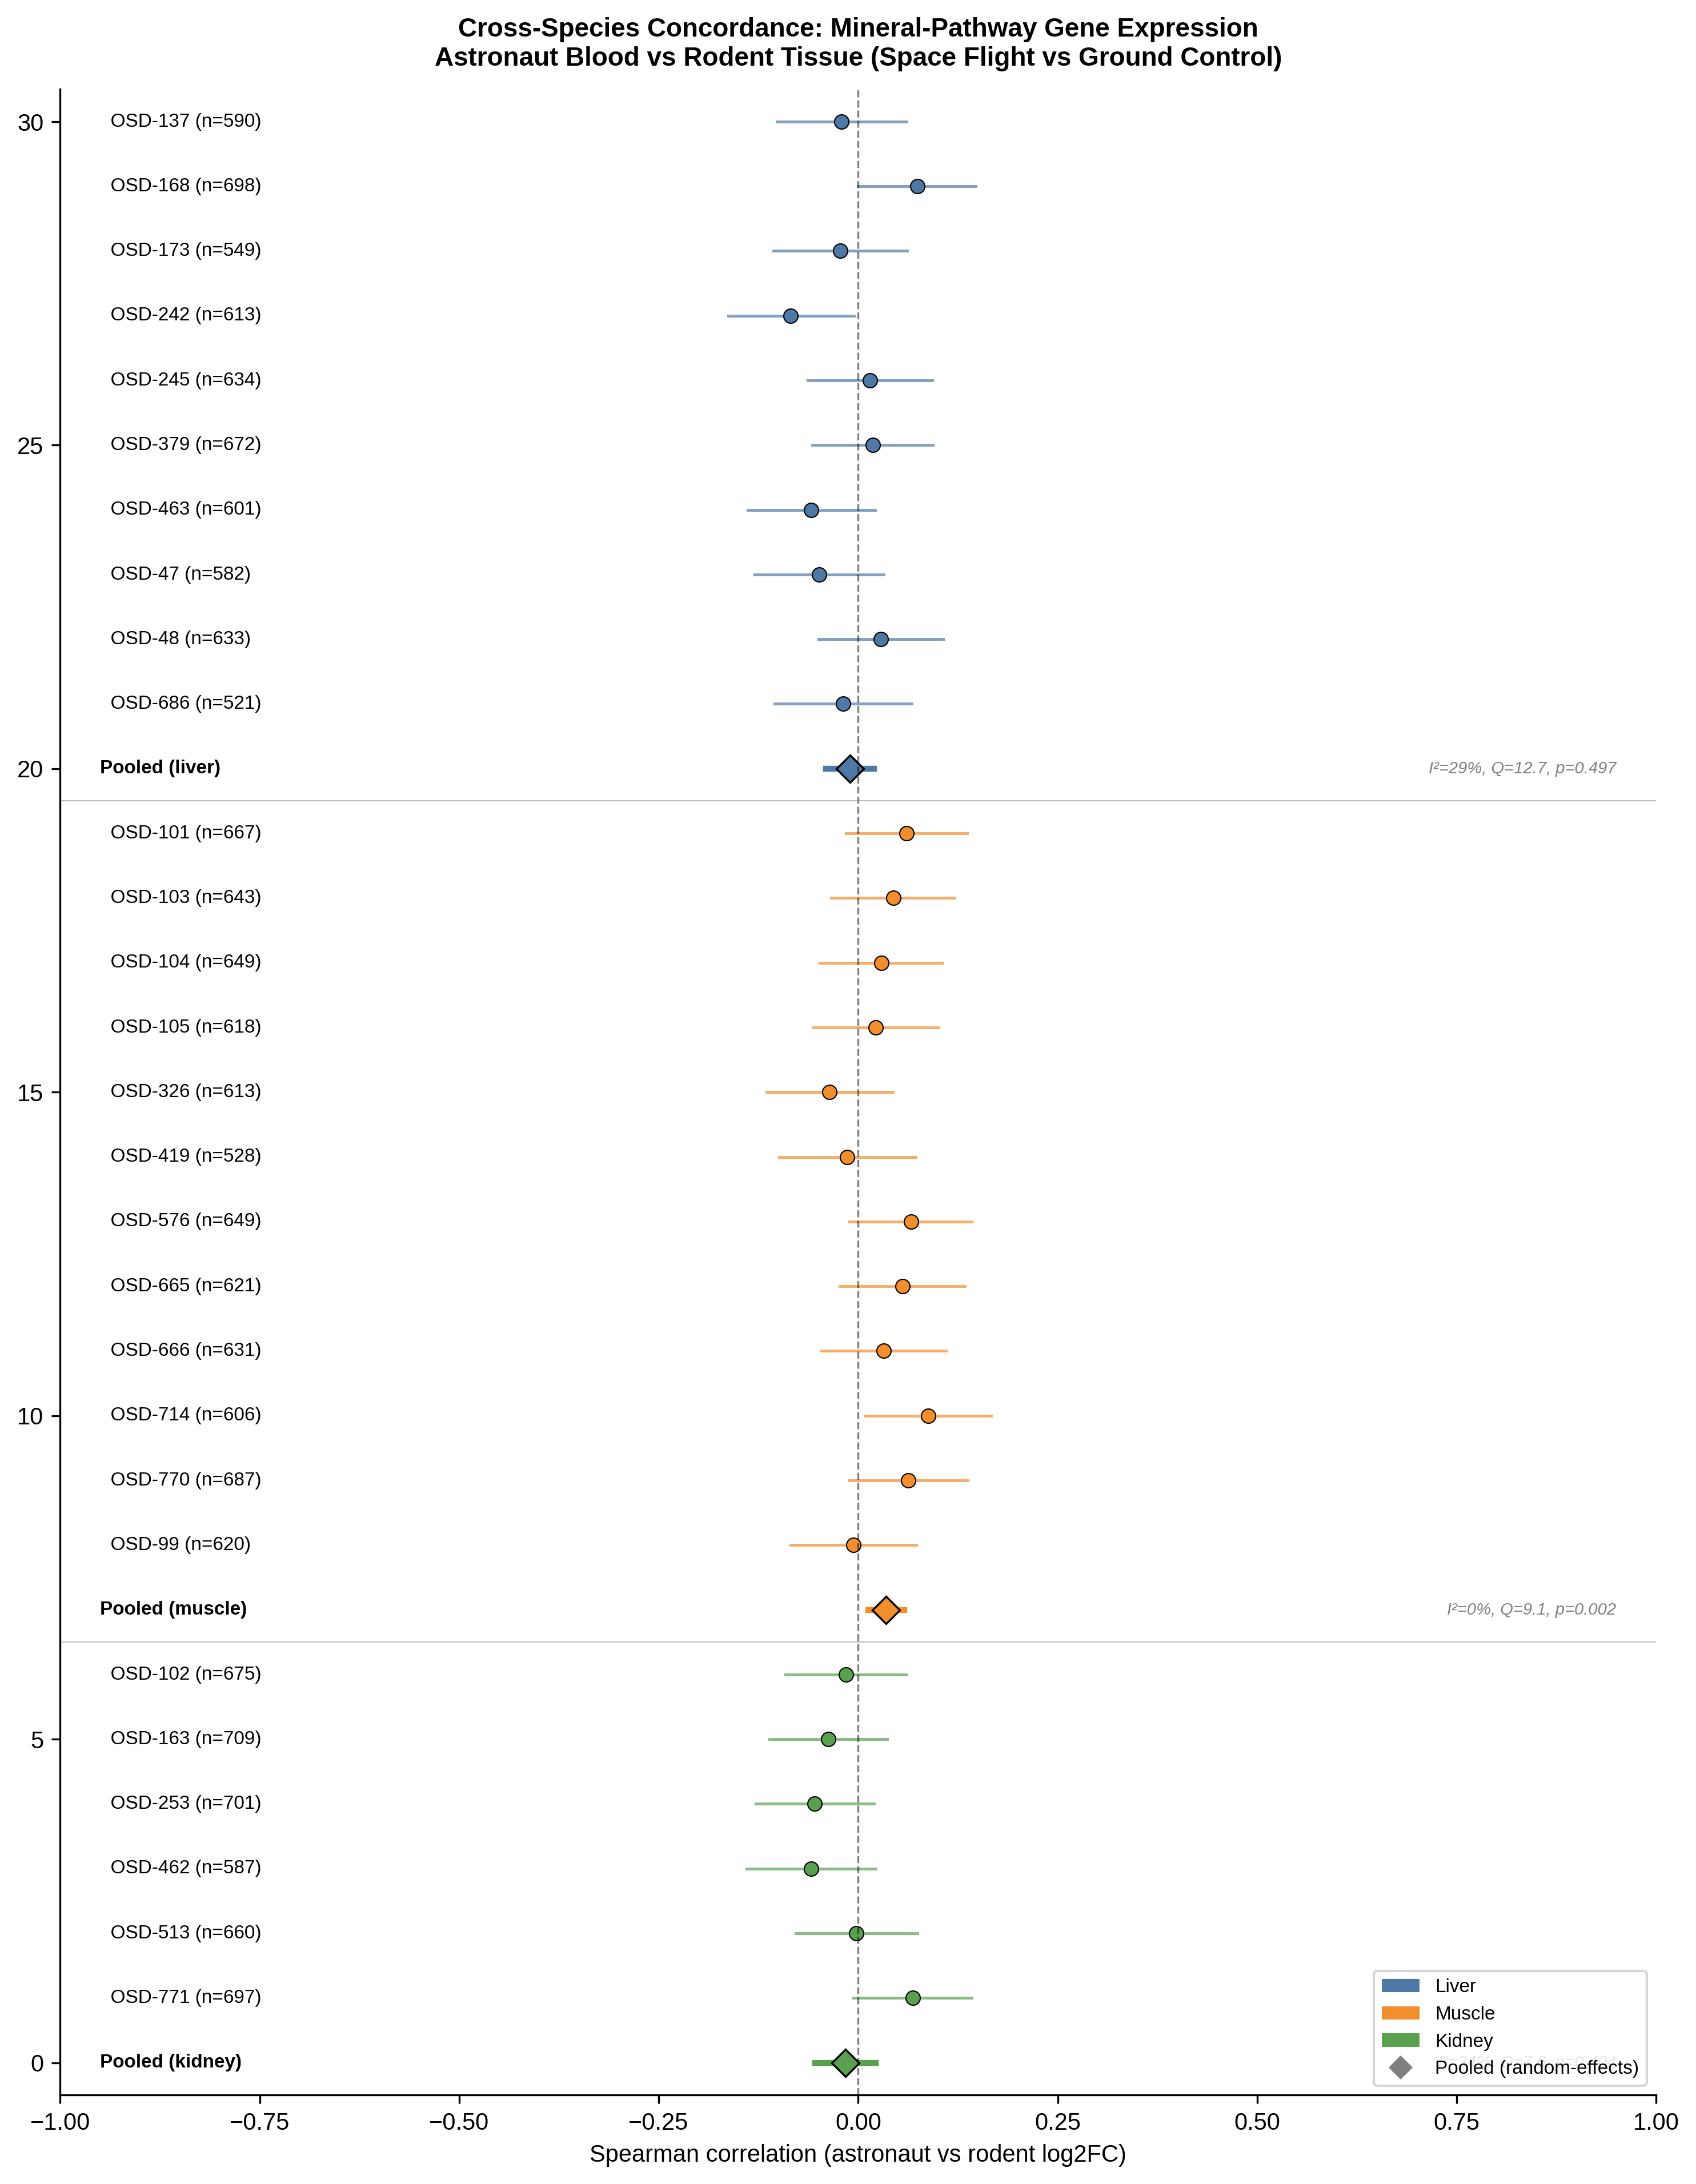
\includegraphics[width=\textwidth]{figures/figS3_forest_cross_species.png}
\caption{}
\end{subfigure}
\hfill
\begin{subfigure}{0.43\textwidth}
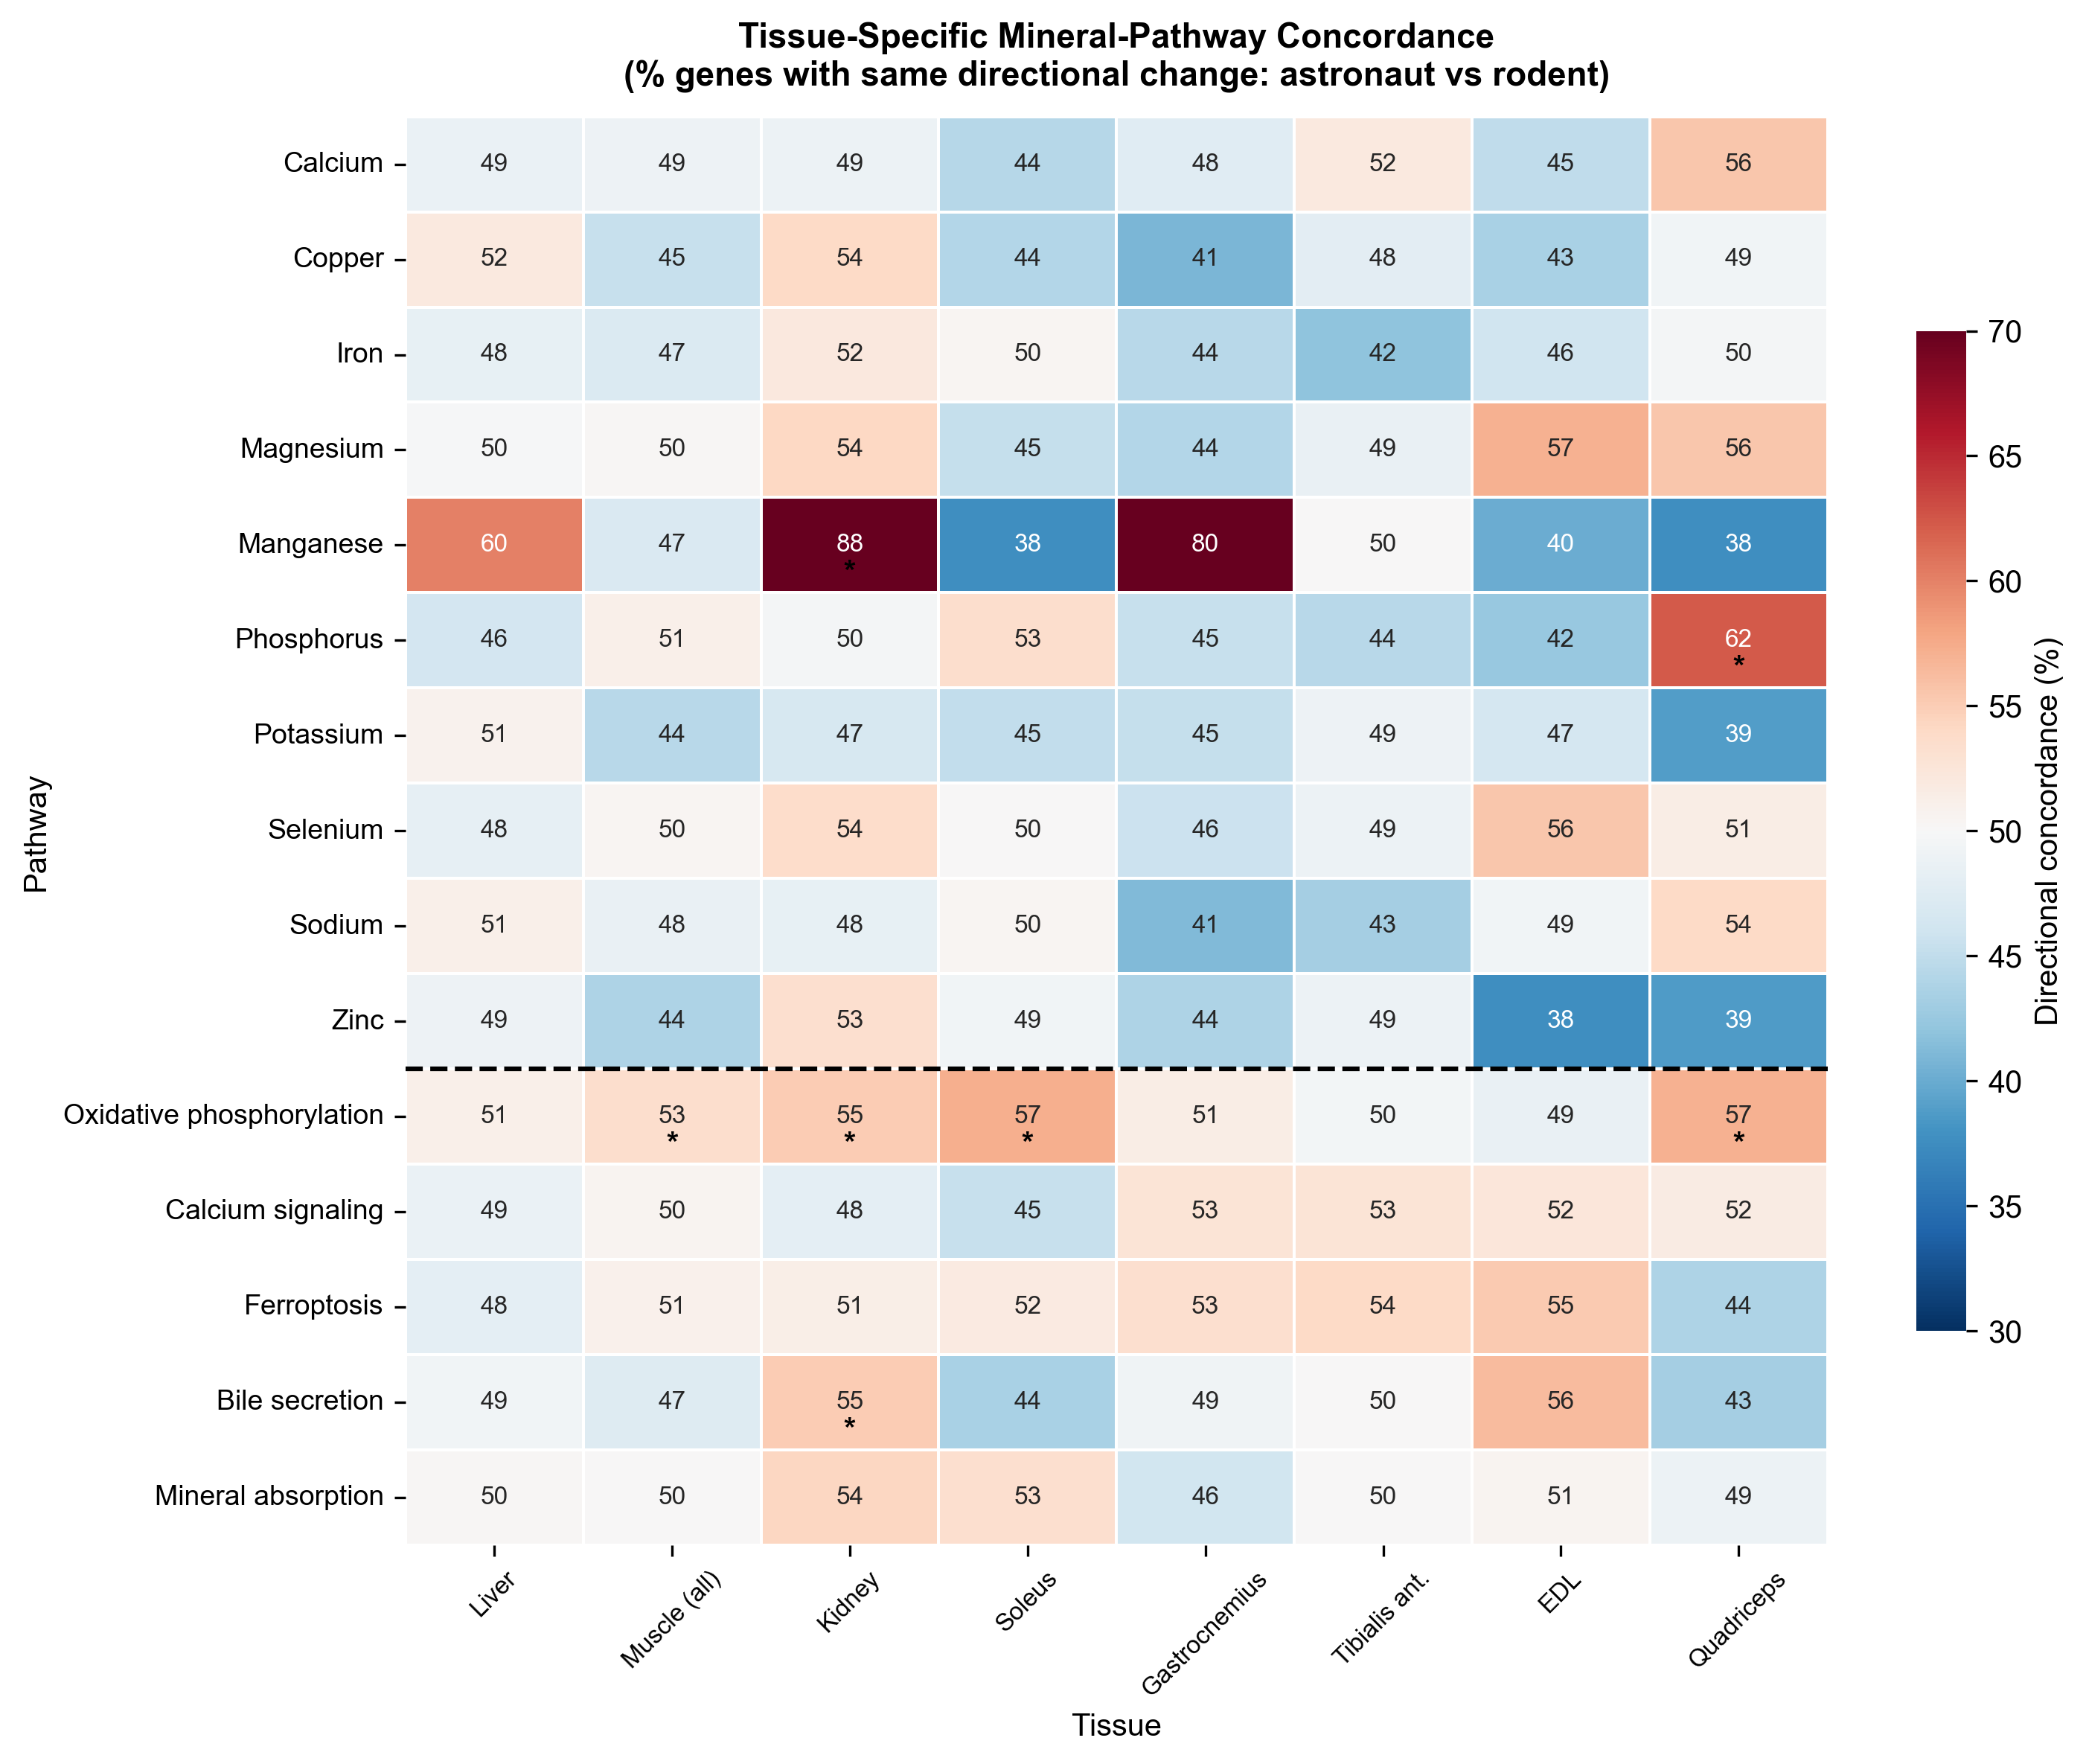
\includegraphics[width=\textwidth]{figures/figS4_tissue_pathway_heatmap.png}
\caption{}
\end{subfigure}
\caption{Cross-species meta-analysis of mineral-pathway concordance. (a) Forest plot showing Fisher $z$ random-effects pooled correlation (astronaut blood vs.\ rodent tissue) by tissue type. Diamond width represents study weight; horizontal lines show 95\% CI. (b) Tissue $\times$ pathway heatmap showing concordance proportions for each mineral pathway across tissues.}
\label{fig:cross_species}
\end{figure}

The muscle-specific concordance pattern supports the hypothesis that skeletal muscle serves as a primary sensor and responder to mineral-pathway disruption in microgravity, consistent with the known effects of mechanical unloading on skeletal muscle\textsuperscript{10}. The absence of liver and kidney concordance likely reflects tissue-specific mineral handling and the confounding effects of comparing peripheral blood (astronaut) with internal organs (rodent). The cross-species scatter plot is provided in Supplementary Figure~S5, and the full meta-analysis summary in Table~\ref{tab:meta_summary}.

\begin{table}[H]
\centering
\caption{Cross-species meta-analysis summary by tissue. Fisher $z$ random-effects pooled correlation between astronaut peripheral blood and rodent tissue mineral-pathway log$_2$FC values.}
\label{tab:meta_summary}
\begin{tabular}{lrrrrr}
\toprule
\textbf{Tissue} & \textbf{$k$} & \textbf{Pooled $r$} & \textbf{95\% CI} & \textbf{$p$-value} & \textbf{$I^2$ (\%)} \\
\midrule
Liver & 10 & $-0.010$ & $[-0.040, 0.020]$ & 0.497 & 29.3 \\
Muscle (all) & 12 & 0.035 & $[0.012, 0.058]$ & 0.002 & 0.0 \\
\quad Soleus & 3 & 0.059 & $[0.015, 0.104]$ & 0.009 & 0.0 \\
\quad EDL & 2 & 0.025 & $[-0.035, 0.085]$ & 0.415 & 14.2 \\
\quad Gastrocnemius & 2 & 0.026 & $[-0.047, 0.099]$ & 0.479 & 38.7 \\
\quad Quadriceps & 3 & 0.014 & $[-0.035, 0.062]$ & 0.573 & 13.4 \\
\quad Tibialis anterior & 2 & 0.045 & $[-0.010, 0.100]$ & 0.111 & 0.0 \\
Kidney & 6 & $-0.016$ & $[-0.054, 0.022]$ & 0.404 & 33.8 \\
All studies & 28 & 0.008 & $[-0.010, 0.025]$ & 0.405 & 30.8 \\
\bottomrule
\end{tabular}
\end{table}

\subsection{Systems biology integration}

A composite systems biology atlas (Figure~\ref{fig:atlas}) integrates KEGG pathway expression changes, mineral-gene set sizes, up/down-regulated DE gene counts per mineral, cross-species concordance, and the top 25 mineral-pathway DE genes into a multi-panel summary. The atlas reveals that copper and calcium pathways show the most consistent dysregulation across omics layers; in the calcium set this reflects down-regulation of the calcium-binding S100 proteins alongside calcium signaling genes with the largest individual fold changes. Iron metabolism genes emerge as a connecting thread: they are differentially expressed (ALAS2, HFE, GLRX5), enriched in ML stability-selected features (HFE 88\%, SLC11A2 81\%, ALAS2 69\%), and show concordant directional changes in rodent muscle. The mineral--gene--pathway network (Supplementary Figures~S6--S8) visualizes these connections.

\begin{figure}[H]
\centering
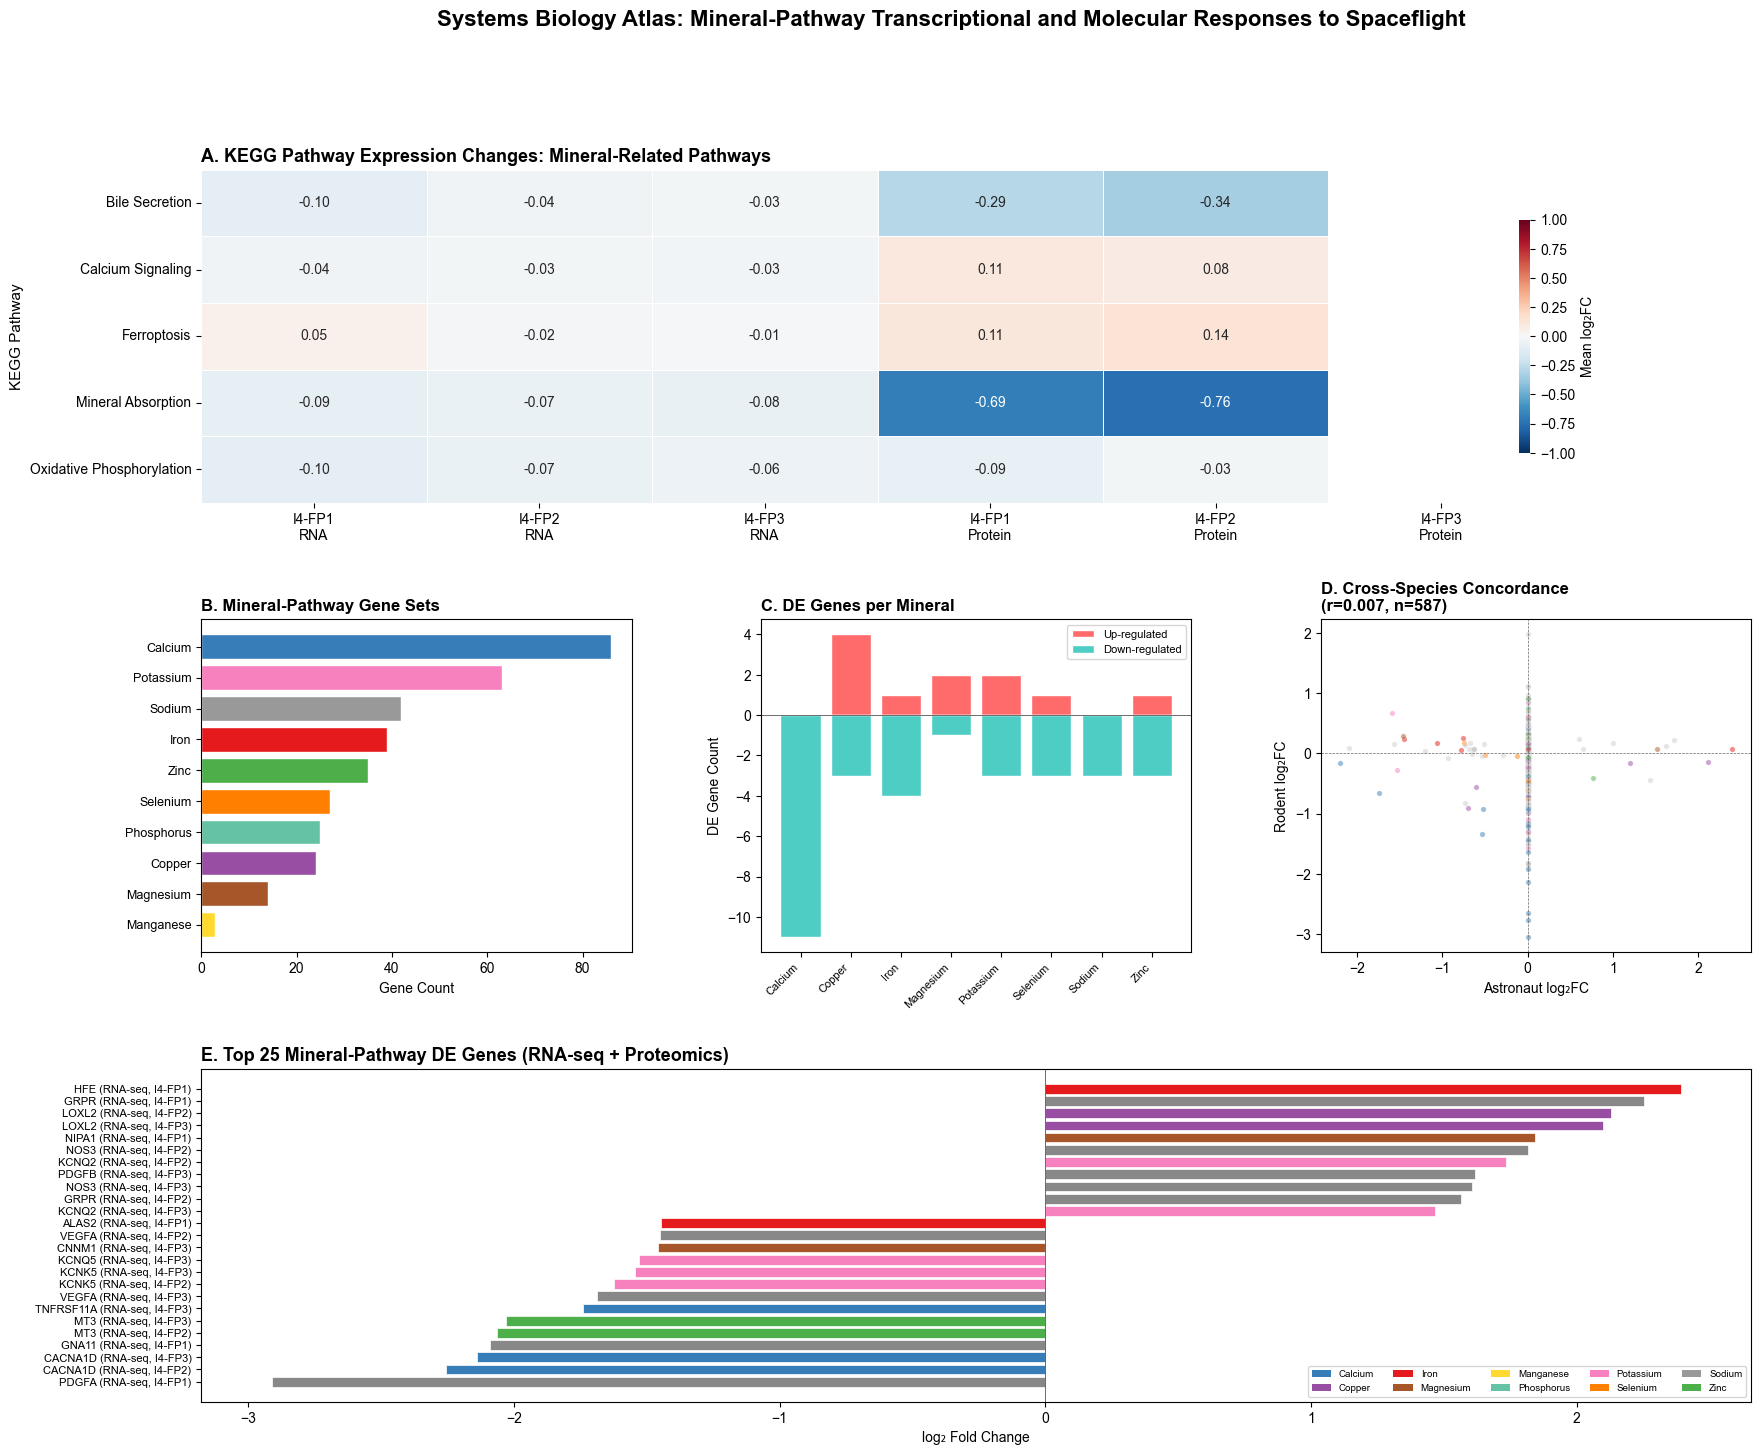
\includegraphics[width=\textwidth]{figures/fig8_systems_biology_atlas.png}
\caption{Systems biology atlas. (A) KEGG pathway mean log$_2$FC across comparisons (RNA-seq and proteomics). (B) Gene counts per mineral gene set. (C) Up/down-regulated DE genes per mineral. (D) Cross-species concordance scatter (astronaut vs.\ rodent log$_2$FC). (E) Top 25 mineral-pathway DE genes with mineral color coding.}
\label{fig:atlas}
\end{figure}

% ════════════════════════════════════════════════════════════════════
% DISCUSSION
% ════════════════════════════════════════════════════════════════════
\section{Discussion}

This study demonstrates that integrating a population reference baseline (NHANES, $n = 5{,}748$) with multi-omics astronaut data ($n = 4$) reveals mineral-pathway deviations that are invisible to within-subject analysis alone. By converting astronaut clinical measurements to population-referenced z-scores and percentile ranks, we identified markers that deviate significantly from normal population distributions --- a framing that addresses the fundamental limitation of interpreting $n = 4$ data without external context.

\subsection{Population-deviating markers: pre-existing vs.\ spaceflight-induced}

A key finding is that several population-deviating markers show deviations at pre-flight baseline. Calcium z-scores were elevated at L-92 ($d = 1.30$) and L-44 ($d = 1.92$), indicating that astronaut calcium levels sit above the 95th population percentile even before spaceflight. This pre-existing deviation may reflect the self-selection of astronauts into physically fit, nutritionally optimized individuals whose mineral status differs from the general population. MPV elevation ($d = 1.73$--$2.47$) was similarly persistent across all timepoints, suggesting a crew-level hematological characteristic rather than a spaceflight effect. These findings underscore the importance of population baselines: without NHANES, these elevated values would appear unremarkable in within-subject comparisons.

In contrast, bicarbonate depression showed a pattern consistent with both pre-existing deviation ($d = -1.24$ at L-92) and post-flight exacerbation ($d = -1.78$ at R+194), suggesting that while astronauts start below population norms, spaceflight may further suppress bicarbonate. Potassium showed a transient elevation at R+45 ($d = 1.79$) that did not survive multiple testing correction, potentially reflecting post-flight fluid rebalancing.

\subsection{Transcriptomic correlates of clinical deviations}

The population-deviating clinical markers show plausible transcriptomic correlates. The down-regulation of CACNA1D ($\log_2\text{FC} = -2.25$), the largest fold change observed, aligns with the elevated serum calcium: cellular down-regulation of calcium channels may represent an adaptive response to sustained extracellular calcium elevation. The iron pathway changes --- ALAS2 down-regulation ($\log_2\text{FC} = -1.45$) and HFE up-regulation ($\log_2\text{FC} = 2.39$) --- are consistent with suppressed erythropoiesis and altered iron sensing, aligning with the modest hemoglobin and RBC deviations from population norms. KCNQ2 up-regulation ($\log_2\text{FC} = 1.73$) may reflect compensatory transcriptional response to potassium shifts.

The ML stability-selected features provide an independent line of evidence: iron metabolism genes (HFE, SLC11A2, ALAS2, PCBP2) were consistently selected across LOO folds, bridging the clinical hematology findings with the transcriptomic response. The potassium channel gene KCNE1 (94\% selection frequency) connects the regression finding (potassium $r = 0.50$) with the classification analysis.

\subsection{Cross-species concordance: muscle as mineral sensor}

The 28-dataset meta-analysis revealed that skeletal muscle --- particularly the soleus --- shows significant concordance with astronaut mineral-pathway responses, while liver and kidney do not. This tissue-specific pattern is biologically plausible: the soleus is a postural muscle that undergoes profound atrophy in microgravity\textsuperscript{10}, and muscle tissue is a major reservoir of intracellular minerals (particularly magnesium and potassium). The concordance effect sizes are small ($r = 0.035$--$0.059$), which is expected given the differences in species (human vs.\ mouse), tissue (blood vs.\ muscle), mission duration (3 days vs.\ 21--90 days), and spaceflight environment (LEO vs.\ ISS). Nevertheless, the statistical significance ($p = 0.002$--$0.009$) across 12 independent muscle datasets provides robust evidence for a conserved mineral-pathway response in skeletal muscle.

\subsection{Limitations}

Several limitations must be acknowledged. First, the astronaut sample size ($n = 4$) is severely underpowered; one-sample tests at each timepoint have minimal statistical power, and we emphasize effect sizes over $p$-values. Second, exact age and sex of individual crew members were not available in the provided dataset; the all-sexes age 40--60 reference was used as the primary baseline. Third, NHANES uses a complex survey design; we used unweighted statistics for reference interval derivation, which is standard practice but may slightly bias population estimates. Fourth, the cross-species comparison is confounded by tissue, mission duration, and species differences. Fifth, the SVM classification AUC $= 1.0$ result must be interpreted with caution due to the non-standard permutation null distribution caused by class weighting. Sixth, the regression $R^2$ values are low (0.12--0.19), indicating that mineral-pathway gene expression explains only a modest fraction of serum mineral variance. Seventh, this is an observational study; no causal inference about spaceflight effects on mineral homeostasis can be drawn.

% ════════════════════════════════════════════════════════════════════
% METHODS
% ════════════════════════════════════════════════════════════════════
\section{Methods}

\subsection{NHANES data acquisition and reference construction}

Three consecutive NHANES cycles (2013--2014, 2015--2016, 2017--2018) were downloaded from the CDC website (\texttt{https://wwwn.cdc.gov/Nchs/Nhanes/}). For each cycle, the Standard Biochemistry Profile (BIOPRO), Complete Blood Count with 5-part differential (CBC), and Demographics (DEMO) XPT files were retrieved and parsed using \texttt{pandas.read\_sas(format='xport')}. Files were merged on the participant identifier (SEQN). The reference population was restricted to adults aged 40--60 years (all sexes), yielding 5,748 participants. Reference statistics (mean, SD, median, percentiles P1--P99) were computed per variable for all sexes combined and stratified by sex. The 95\% reference interval was defined as P2.5--P97.5.

\subsection{Astronaut data acquisition}

Astronaut data were retrieved from the NASA OSDR REST API (\texttt{https://visualization.osdr.nasa.gov/biodata/api}). Studies included: OSD-569 (RNA-seq), OSD-571 (proteomics and metabolomics DE), OSD-575 (Comprehensive Metabolic Panel and CBC), and OSD-656 (urine immune panel). All data correspond to the Inspiration4 mission with four civilian astronauts (C001--C004) sampled at seven timepoints: L-92, L-44, L-3 (pre-flight), R+1 (return/flight), R+45, R+82, R+194 (post-flight). Clinical chemistry variables (calcium, potassium, sodium, chloride, bicarbonate) were from the CMP panel; hematological variables (hemoglobin, hematocrit, RBC, MCH, MCHC, MCV, WBC, RDW, platelets, MPV) were from the CBC panel.

\subsection{Population-referenced analysis}

Each astronaut measurement was converted to a z-score: $z = (x_{\text{astro}} - \mu_{\text{NHANES}}) / \sigma_{\text{NHANES}}$, where $\mu$ and $\sigma$ are the NHANES age 40--60 all-sexes mean and SD. Empirical percentile ranks were computed using the NHANES reference distribution. Measurements falling outside P2.5--P97.5 were flagged as outside the reference interval. One-sample $t$-tests (astronaut values vs.\ NHANES mean) and Wilcoxon signed-rank tests were performed at each timepoint. Cohen's $d$ was computed as $(\bar{x}_{\text{astro}} - \mu_{\text{NHANES}}) / \sigma_{\text{NHANES}}$. Benjamini--Hochberg FDR correction was applied across all 105 tests (15 variables $\times$ 7 timepoints). Three implausible values (C003 at L-92: MPV = 330 fL, RDW = 32.4\%, platelets = 12.9 $\times$ 10$^3$/uL) were identified as data entry errors and excluded.

\subsection{Mineral-pathway gene set construction}

Curated mineral homeostasis gene sets for 10 minerals (calcium, iron, magnesium, zinc, copper, selenium, potassium, sodium, phosphorus, manganese) were compiled from KEGG pathway hsa04978 (Mineral absorption), UniProt, HGNC, and published literature. Five KEGG pathways were included: hsa04978 (61 genes), hsa04020 (254 genes), hsa04216 (42 genes), hsa00190 (138 genes), and hsa04976 (90 genes). The final gene set comprised 801 unique genes, with 784 mapped to the astronaut RNA-seq feature space after ENSEMBL-to-HGNC symbol mapping via the mygene.info API (73.6\% mapping rate).

\subsection{RNA-seq differential expression}

The I4 RNA-seq data included two DE methods: DESeq2 and a pipeline-transcriptome-de approach. The pipeline-transcriptome-de method yielded meaningful fold changes (range $-2.91$ to $2.39$) and was used as the primary DE method, as DESeq2 log$_2$FC values were uniformly near zero. Three flight comparisons were analyzed: I4-FP1 (R+1 vs.\ pre-flight), I4-FP2 (R+1/R+45/R+82 vs.\ pre-flight), and I4-FP3 (all post-flight vs.\ pre-flight). Significant genes were defined as $|\log_2\text{FC}| > 0.5$ and $p < 0.05$.

\subsection{Proteomics and metabolomics}

Proteomics DE was performed using limma (I4-FP1 and I4-FP2 comparisons) with 3,285 proteins. Metabolomics DE included 2,624 metabolites across two comparisons. Proteomics data contained gene symbols; metabolomics data used metabolite identifiers.

\subsection{Gene set enrichment analysis}

GSEA was performed with \texttt{gseapy} (Python; preranked mode, 1,000 permutations, seed 42). RNA-seq genes were ranked by $\mathrm{sign}(\log_2\text{FC}) \times -\log_{10}(p)$ for each flight comparison, and proteins by the limma $t$-statistic for I4-FP1 and I4-FP2. Gene sets included the 10 mineral-specific gene sets and 5 KEGG pathway gene sets. Normalized enrichment scores (NES), NOM $p$-values, and FDR $q$-values were reported.

\subsection{Machine learning: regression}

Feature matrices were constructed from RNA-seq count data restricted to 784 mineral-pathway genes, log$_2$(counts + 1) transformed, with the top 200 genes by variance selected. Four regressors (Ridge, SVR-Linear, SVR-RBF, RandomForest) predicted serum calcium, potassium, sodium, and hemoglobin under LOO-CV ($n = 16$). Performance was assessed by Pearson $r$ and $R^2$. Permutation importance (20 repeats) identified key predictive genes.

\subsection{Machine learning: classification}

Class-weighted elastic-net logistic regression (\texttt{LogisticRegression(penalty='elasticnet', class\_weight='balanced', solver='saga')}) was applied with nested LOO-CV. The outer loop held out 1 of 16 samples (4 flight, 12 ground); the inner loop (3-fold stratified) selected hyperparameters (C $\in$ \{0.01, 0.05, 0.1, 0.5, 1.0\}, l1\_ratio $\in$ \{0.1, 0.3, 0.5, 0.7, 0.9\}). StandardScaler was fit inside each fold. SVM-RBF with class weights was included as a non-linear baseline. A 500-permutation test shuffled labels and reran the full LOO-CV to generate the null distribution. Stability selection tracked gene selection frequency across LOO folds.

\subsection{Cross-species meta-analysis}

Twenty-eight rodent spaceflight datasets were retrieved from the NASA OSDR, comprising 10 liver, 12 muscle (EDL, gastrocnemius, quadriceps, soleus, tibialis anterior), and 6 kidney datasets. For each dataset, flight vs.\ ground control DE was computed using Welch's $t$-tests with Benjamini--Hochberg correction. Mouse ENSEMBL IDs were mapped to human gene symbols via mygene.info homologene data. Fisher $z$ random-effects meta-analysis was performed by tissue type, pooling individual study $z$-transformed correlations between astronaut and rodent mineral-pathway log$_2$FC values. Heterogeneity was assessed using Cochran's $Q$ and $I^2$.

\subsection{Statistical methods}

All statistical analyses were performed in Python 3.11 using \texttt{scipy}, \texttt{statsmodels}, \texttt{scikit-learn}, and \texttt{pandas}. Multiple testing correction used Benjamini--Hochberg FDR. Effect sizes were reported as Cohen's $d$ for group comparisons and Pearson $r$ for correlations. Reference intervals were defined as P2.5--P97.5 (95\% interval) and P5--P95 (90\% interval).

\subsection{Reproducibility}

All analysis scripts, processed data, figures, and a data dictionary are available in a FAIR-compliant Zenodo package. Scripts are numbered 01--11, covering data acquisition, processing, ML analysis, visualizations, cross-species meta-analysis, NHANES integration, and supplementary outputs. Python 3.11 with \texttt{scipy}, \texttt{scikit-learn}, \texttt{pandas}, \texttt{matplotlib}, and \texttt{statsmodels} was used throughout.

% ════════════════════════════════════════════════════════════════════
% REFERENCES
% ════════════════════════════════════════════════════════════════════
\section*{References}

\begin{thebibliography}{99}

\bibitem{williams2009}
Williams D, Kuipers A, Mukai C, Thirsk R. Acclimation during space flight: effects on human physiology. \textit{CMAJ}. 2009;180(13):1317--1323. doi:10.1503/cmaj.090628

\bibitem{norsk2015}
Norsk P, Asmar A, Damgaard M, Christensen NJ. Fluid shifts, vasodilatation and ambulatory blood pressure reduction during long duration spaceflight. \textit{J Physiol}. 2015;593(3):573--584. doi:10.1113/jphysiol.2014.284869

\bibitem{stein2002}
Stein TP. Space flight and oxidative stress. \textit{Nutrition}. 2002;18(10):867--871. doi:10.1016/S0899-9007(02)00938-3

\bibitem{overbey2024}
Overbey EG, Kim J, Tierney BT, et al. The Space Omics and Medical Atlas (SOMA) and international astronaut biobank. \textit{Nature}. 2024;632(8027):1145--1154. doi:10.1038/s41586-024-07639-y

\bibitem{cdc_nhanes}
Centers for Disease Control and Prevention (CDC). National Health and Nutrition Examination Survey. Hyattsville, MD: National Center for Health Statistics. Available at: \texttt{https://www.cdc.gov/nchs/nhanes/}.

\bibitem{smith2002iron}
Smith SM. Red blood cell and iron metabolism during space flight. \textit{Nutrition}. 2002;18(10):864--866. doi:10.1016/S0899-9007(02)00912-7

\bibitem{smithmungo1998}
Smith-Mungo LI, Kagan HM. Lysyl oxidase: properties, regulation and multiple functions in biology. \textit{Matrix Biol}. 1998;16(7):387--398. doi:10.1016/S0945-053X(98)90012-9

\bibitem{wang2018}
Wang S, Song R, Wang Z, et al. S100A8/A9 in inflammation. \textit{Front Immunol}. 2018;9:1298. doi:10.3389/fimmu.2018.01298

\bibitem{hughesfulford2004}
Hughes-Fulford M. Signal transduction and mechanical stress. \textit{Sci STKE}. 2004;2004(249):re12. doi:10.1126/stke.2492004re12

\bibitem{fitts2010}
Fitts RH, Trappe SW, Costill DL, et al. Prolonged space flight-induced alterations in the structure and function of human skeletal muscle fibres. \textit{J Physiol}. 2010;588(18):3567--3592. doi:10.1113/jphysiol.2010.188508

\bibitem{smith2005}
Smith SM, Wastney ME, O'Brien KO, et al. Bone markers, calcium metabolism, and calcium kinetics during extended-duration space flight on the Mir space station. \textit{J Bone Miner Res}. 2005;20(2):208--218. doi:10.1359/JBMR.041105

\bibitem{smith2015}
Smith SM, Heer M, Shackelford LC, et al. Bone metabolism and renal stone risk during International Space Station missions. \textit{Bone}. 2015;81:712--720. doi:10.1016/j.bone.2015.10.002

\bibitem{hedges1985}
Hedges LV, Olkin I. \textit{Statistical Methods for Meta-Analysis}. Orlando: Academic Press; 1985.

\bibitem{benjamini1995}
Benjamini Y, Hochberg Y. Controlling the false discovery rate: a practical and powerful approach to multiple testing. \textit{J R Stat Soc B}. 1995;57(1):289--300. doi:10.1111/j.2517-6161.1995.tb02031.x

\bibitem{subramanian2005}
Subramanian A, Tamayo P, Mootha VK, et al. Gene set enrichment analysis: a knowledge-based approach for interpreting genome-wide expression profiles. \textit{Proc Natl Acad Sci USA}. 2005;102(43):15545--15550. doi:10.1073/pnas.0506580102

\bibitem{chu2010}
Chu SG, Becker RC, Berger PB, et al. Mean platelet volume as a predictor of cardiovascular risk: a systematic review and meta-analysis. \textit{J Thromb Haemost}. 2010;8(1):148--156. doi:10.1111/j.1538-7836.2009.03584.x

\end{thebibliography}

\end{document}
